%
% Copyright (c) 2008  Betti "Osterholz
%
% Permission is granted to copy, distribute and/or modify this document
% under the terms of the GNU Free Documentation License, Version 1.2 or
% any later version published by the Free Software Foundation;
% with no Invariant Sections, no Front-Cover Texts, and no Back-Cover Texts.
%
% A copy of the license is included in the file ``fdl.tex'' .
%

%path for pictures
\graphicspath{{./material_sprachbeschreibung/}}
\graphicspath{{./material_sprachbeschreibung/}{../material_sprachbeschreibung}}


\newpage
\part{Fib-Sprachbeschreibung}
\label{partFibLanguage}

In diesem Teil werden die Elemente der Fib-Multimediasprache vorgestellt und einige grundlegende Aussagen zur Fib-Multimediasprache getroffen.


\section{Anforderungen}
\label{secFibLanguageRequirements}

Da die klassische Bitdarstellung bei genetischen Algorithmen eine geringe Performance erwarten l"asst,  aber gerade wegen der Komplexit"at des Problems eine m"oglichst hohe Performance von N"oten ist, wird eine angepasste Problemdarstellung (Multimediabeschreibungssprache) gew"ahlt.

Die Multimediabeschreibungssprache Fib sollte m"oglichst einfach gehalten werden, mit m"oglichst wenigen Alternativen, da mit dem Anstieg der zur Auswahl stehenden Alternativen auch die Anzahl der Alternativen bei der Anwendung der genetischen Operationen steigt und damit wahrscheinlich der Rechenaufwand und der Realisierungsaufwand.

Dennoch sollen mit der Multimediabeschreibungssprache kompakte Ausdr"ucke f"ur ``normale'' (in der Anwendung auftretende) Multimediaobjekte m"oglich sein. Es soll also gute Komprimierungsm"oglichkeiten f"ur ``normale'' Multimediaobjekte geben. Das beinhaltet, dass Zusammenh"ange (z. B. Farbverl"aufe in einer Fl"ache) zwischen Teilen (z. B. Pixeln der Fl"ache) eines Multimediaobjekts m"oglichst einfach dargestellt werden k"onnen.

Die Sprache sollte eindeutig, reproduzierbar und auswertbar sein, so dass ein Ausdruck immer zum gleichen Objekt ausgewertet wird. Bei der Eindeutigkeit und Reproduzierbarkeit k"onnen in der Implementierung Abstriche gemacht werden (z. B. wegen unterschiedlichen Rundungsfehlern auf unterschiedlichen Architekturen), wenn das erzeugte Multimediaobjekt so gut wie immer (in beispielsweise dem 0,999999sten Anteil der F"alle) dem original Multimediaobjekt sehr "ahnlich ist. Die g"ultigen Sprachobjekte m"ussen jedoch immer auswertbar sein, da sonst Einschr"ankungen bei den genetischen Operatoren, die sie erzeugen, gemacht werden m"ussten oder nicht auswertbare Objekte entstehen k"onnten.

Es soll mit der Multimediabeschreibungssprache m"oglich sein, zumindest alle m"oglichen Rastergrafiken darzustellen.
Die Erzeugung einer Rastergrafik aus einem Fib-Multimediaobjekt in der Multimediabeschreibungssprache soll nachvollziehbar sein. Das hei"st, die Multimediabeschreibungssprache soll die Unterscheidung einzelner Objekte und deren Zusammenhang unterst"utzen.

Die Multimediaprogramme ver"andernden genetischen Operationen sollten, wenn m"oglich, das Programm so ver"andern, dass im Hypothesenraum der Multimediaprogramme diese Operatoren einen Gradientenanstieg erm"oglichen. Durch Ausf"uhrung mehrerer Operatoren sollte also die Hypothese, die das Multimediaprogramm darstellt, allm"ahlich verbessert werden k"onnen.


\section{Die Multimediabeschreibungssprache}

Die Multimediabeschreibungssprache tr"agt den Namen Fib (f"ur funktionale Interpretation von Bildern oder ``functional interpretation of bictures/bitmaps''). Dieser Namen leitet sich noch aus der ersten Version der Multimediabeschreibungssprache her, als sie nur zum Abspeichern von Bildern geeignet war.

Durch einige zus"atzliche Elemente wurde die Multimediabeschreibungssprache so erweitert, dass sie beliebige Multimediadaten abspeichern kann. Die einzige Einschr"ankung bez"uglich der Multimediadaten ist, dass sie als Eigenschaften von Punkten eines endlichen, euklidischen und diskreten (es gibt kleinste Einheiten) Raumes darstellbar sind.

Fib ist eine Vektordarstellung von Multimediadaten, also eine Darstellung von Multimediadaten mit Hilfe von Objekten.
Als Grundger"ust dient ein Baum. Die Bl"atter sind Endpunkte, die f"ur die Darstellung von bzw. Zuordnung zu Punkten oder Teilmultimediaobjekten dienen. In den "Asten und der Ausrichtung dieser, welche z. B. am weitesten links stehen, werden Darstellungsparameter oder Eigenschaften der Bl"atter kodiert, z. B. wie oft es dargestellt wird und mit welcher Farbe.

Jeder Knoten des Baums ist ein Fib-Element. Der Baum wird von der Wurzel zu den Bl"attern ausgewertet, wobei die Elemente die Auswertung beeinflussen.

Ein vollst"andiges Fib-Objekt (Baum) repr"asentiert ein Multimediaobjekt.

Ein g"ultiges Fib-Objekt (Baum) ist zyklenfrei, um eine endliche Verarbeitungszeit zu gew"ahrleisten.
Die Elemente der Multimediabeschreibungssprache orientieren sich dabei etwas an den "ublichen imperativen Programmiersprachen (z. B. C++, Java).

Alle Einheiten sind auf Grundlage des Internationalen Einheitensystems (SI) anzugeben.

Beim Auswerten eines Fib-Objekts werden f"ur das Multimediaobjekt alle Punkte mit ihren Eigenschaften ermittelt. Ein ausgewertetes Multimediaobjekt enth"alt damit nur eine Liste von konkreten Punkten und ihren Eigenschaften, so dass es direkt angezeigt (durch Darstellung der Eigenschaften an den Punkten/Koordinaten) bzw. ausgewertet werden kann.

Im Nachfolgenden wird als ``oben'' im Fib-Objekt die Richtung bezeichnet, in der die Wurzel des Baums liegt. Die Richtung ``unten'' ist damit die entgegengesetzte Richtung (also weg von der Wurzel).


\section{Elemente der Fib-Multimediabeschreibungssprache}
\label{secFibElements}

In diesem Abschnitt werden die Elemente beschrieben, aus denen die Fib-Multi\-media\-beschrei\-bungs\-sprache aufgebaut ist.

Im Nachfolgendem bezeichnet $Obj$ ein Fib-Objekt.



\subsection{Vektoren}\index{Vektoren|(}

Vektoren dienen zum Bereitstellen von numerischen Werten. Es gibt verschiedene Typen von Vektoren (z. B. Positionsvektor, Bereichsvektor oder Eigenschaftsvektor f"ur RGB-Farben). Aus dem Typ eines Vektors (und eventuell den Angaben im root-Element) ergeben sich die Anzahl und die Definitionsbereiche der Elemente, die er enthalten kann.
Jedes Vektorelemente ist entweder eine Zahl oder eine Variable, welche weiter oben im Fib-Objekt belegt wird.

Liegt der Werte eines ausgewerteten Elements au"serhalb des Definitionsbereichs, f"ur den das Vektorelement definiert ist, wird dieser Wert auf den n"achsten Wert gerundet, der im Definitionsbereich liegt.
Wenn ein Element des Vektors nicht belegt ist, wird es als der Nullwert des Definitionsbereichs ausgewertet.

Vektoren eines Typs k"onnen nur in einem ganz bestimmten Fib-Element verwendet werden.

Eine Auflistung der m"oglichen Vektoren ist in Tabelle \ref{tableVectorTyps} zu sehen.

\begin{table}[htbp]
\begin{center}
\begin{small}
\begin{tabular}{|p{20mm}|p{35mm}|p{15mm}|p{20mm}|p{15mm}|}\hline
	Vektor & Beschreibung & wird verwendet in Fib-Element & Anzahl Elemente & Typ Elemente \\\hline\hline
	Position & gibt die Position eines Punktes an & $point$ (Punkt) & beliebig (Vektor mit 0 Elementen ist immer m"oglich) & Zahlen\\\hline
	Bereich & gibt die Grenzen eines Teilbereichs (inklusive der Grenzen) an & $area$ (Bereich) & 2 & ganze Zahlen\\\hline
	Eigenschafs\-vektoren (es kann beliebige geben) & definiert die Werte einer Eigenschaft & $property$ (Eigenschaften) & beliebig & Zahlen\\\hline
\end{tabular}
\end{small}
\end{center}
\caption{Vektorentypen}
\label{tableVectorTyps}
\end{table}

\index{Vektoren|)}


\subsection{Punkte}\index{Punktelement|(}
\label{fibPoint}\label{secFibPoint}

\begin{flushleft}
Die Punkte sind die darstellenden Elemente. An ihnen werden die gesetzten Eigenschaften ausgewertet. Punkte dienen als Bl"atter eines Fib-Objekts.

Ein leerer Punkte ``point()'' ist m"oglich. Der leere Punkt hat keine Auswirkungen (alle Eigenschaften gehen verloren). Genutzt werden kann er in Kombination mit anderen Elementen (z. B. dem $if$-Element).

Daneben gibt es auch Punkte mit leerem Positionsvektor ``point(())'', diese erzeugen den Hintergrund (z. B. Hintergrundfarbe).

Die Eigenschaften des Punkts (z. B. Farbe, Ton oder/und Geruch) werden im Ast "uber dem Punkt durch property-Elemente bestimmt.

\bigskip\noindent
Syntax:
$Obj = point( PositionVector )$

\bigskip\noindent
Kurzsyntax:
$Obj = p( PositionVector )$

\bigskip\noindent
Beschreibung der Elemente:
\begin{description}
 \item[$PositionVector$]: die Koordinatenvektor des Punktes
\end{description}

\bigskip\noindent
Beispiel:
\begin{itemize}
 \item $p((10;20))$; Ein Punkt an der Position $(10, 20)$.
 \item $p((10;x))$; Das Symbol $x$ steht f"ur eine Variable, die im Ast zu diesem Punkt belegt werden muss.
 \item $p()$; Der Punkt hat keine Auswirkungen und alle Eigenschaften werden verworfen.
 \item $p(())$; Der Punkt wirkt sich auf den gesamten Hintergrund aus.
\end{itemize}

\end{flushleft}

\index{Punktelement|)}


\subsection{Eigenschaftselement}\index{Eigenschaftselement|(}
\label{fibProperty}\label{secFibProperty}

Mit dem Eigenschaftselement ``property'' werden Eigenschaften f"ur Fib-Objekte gesetzt.

\bigskip\noindent
Syntax:
$Obj = property( ( value_1, ..., value_n)_{name}, Obj_1 ) $

\bigskip\noindent
Kurzsyntax:
$Obj = pr( (value_1, ..., value_n)_{name}, Obj_1 )$

\bigskip\noindent
Beschreibung der Elemente:
\begin{description}
 \item[$name$] Der $name$ gibt den Namen der Eigenschaft an. Er bestimmt den Typ des Vektors. Alle Eigenschaftsvektortypen sollten zum Vektorobertyp ``property'' geh"oren.
 \item[$value_i$] Dies ist der Wert $i$ der Eigenschaft.
 \item[$Obj_1$] Das ist das enthaltende Objekt, f"ur welches die Eigenschaft gesetzt wird.
\end{description}


\begin{small}
\begin{center}
\begin{longtable}{|p{22mm}|p{6mm}|p{5mm}|p{50mm}|p{30mm}|}\hline
	\textbf{Name} & \textbf{Wert} & \textbf{\#El.} & \textbf{Beschreibung} & \textbf{Beispiel} \\\hline\endhead
	whatever & 0 & 0 & Die Eigenschaften des Unterobjekts ist egal. Welche Eigenschaften diesem Unterobjekt auch immer zugeordnet werden, sie sind richtig. & pr( $()_{whatever}$, Obj )\\\hline
	\multicolumn{5}{|c|}{\textbf{Farben}}\\
	\multicolumn{5}{|c|}{(Alle Farben "uberschreiben die f"ur das aktuelle Fib-Objekt gesetzten Farben.)}\\\hline
	colorRGB & 1 & 3 & Farbanteile als Rot-, Gr"un- und Blau-Werte & pr( $(255, 16, 0$ $)_{colorRGB}$, Obj )\\\hline
%TODO?: colorCMYK
	colorGrayscale & 2 & 1 & Helligkeitsanteil & pr( $(25)_{colorGrayscale}$, Obj )\\\hline

	\multicolumn{5}{|c|}{\textbf{weitere Eigenschaften}}\\\hline
	layer & 100 & 1 & Ebenen f"ur die Punkte (niedrige Ebenen werden von h"oheren "uberdeckt) & pr( $(2)_{layer}$, Obj )\\\hline
	transparency & 200 & 1 & Durchsichtigkeitsanteil (f"ur Farben) der Punkte & pr( $(25)_{transparency}$, Obj ) \\\hline
	persistent & 210 & 0 & Diese Eigenschaft ist nur f"ur einen Zeitraum (bzw. der Dimensionsrichtung Zeit) sinnvoll. Raumpunkte mit diese Eigenschaft verlieren ihre anderen Eigenschaften nur, wenn diese zeitlich sp"ater durch jeweils eine Eigenschaft vom gleichen Typ "uberschrieben wird. Dies gilt nat"urlich nur, solange der jeweilige "uberschriebene Punkt die Eigenschaft $persistent$ hat. Sinnvoll ist dies, wenn beispielsweise in einem Film Objekte so lange sichbar sein sollen, wie sie nicht von anderen Objekten "uberschrieben werden. Dann kann das gesamte Fib-Objekt die Eigenschaft $persistent$ bekommen. Wird dann ein Objekt zu einer Zeit definiert und angezeigt, bleibt es in Zukunft solange bestehen, bis es "uberschrieben wird. &  pr( $()_{persistent}$, Obj ) \\\hline

	\multicolumn{5}{|c|}{\textbf{Ton-Eigenschaften}}\\\hline
	sound & 300 & 4 & ein Ton; Die Werte sind: 1. Frequenz in Hertz ($1/s$), 2. Schalldruck in Pascal $Pa$ ($1 Pa= 1 N/m^2$), 3. Phasenverschiebung in Bogenma"s 4. Dauer in Sekunden. Ein Ton wirkt additiv mit anderen T"onen. & pr( $(5000, 40, 0.5, 50$ $)_{sound}$, Obj) \\\hline
	soundPolarized & 301 & $3 + \sharp$ $Dim$ & ein Ton; Die Werte sind: 1. Frequenz in Hertz ($1/s$), 2. Schalldruck in Pascal $Pa$ ($1 Pa= 1 N/m^2$), 3. Phasenverschiebung in Bogenma"s, 4. Dauer in Sekunden, r = $5$ bis ($3 + \sharp Dim$) Polarisierungsanteil (als Winkel in Bogenma"s) in der Dimensionsebene, welche von den jeweiligen Dimensionen $r-4$ und $r-3$ aufgespannt wird. ($\sharp Dim$ ist die Anzahl der Dimensionen.) Die Winkelangabe erfolgt von der $r-3$ Achse in positiver Richtung. Ein Ton wirkt additiv mit anderen T"onen. & pr( $(5000, 40, 2, 0.5, 5$ $)_{soundPolarized}$, Obj) \\\hline

	soundAmplitude & 305 & 3 & die Amplitude eines Tons; Die Werte sind: 1. Schalldruck in Pascal $Pa$ ($1 Pa= 1 N/m^2$), 2. Phasenverschiebung in Bogenma"s 3. Dauer in Sekunden. Ein Ton wirkt additiv mit anderen T"onen. Mit dieser Eigenschaft k"onnen T"one "uber ihre Amplituden mit einer bestimmten Abtastrate aufgebaut werden, wie z. B. im WAVE-Dateiformat. & pr( $( 40, 0.5, 0.0005$ $)_{soundAmplitude}$, Obj) \\\hline

	soundBarrier & 310 & 1 & Geschwindigkeit des Schalls in Meter pro Sekunde ($m/s$); Damit k"onnen Objekte die Akustik ver"andern. & pr( $(343)_{soundBarrier}$, Obj) \\\hline
	soundReflected & 311 & 1 & Anteil des vom Objekt zur"uckgeworfener Schalls; Diese Eigenschaft gilt f"ur die Oberfl"ache/den Rand des Objekts und nicht f"ur alle seine einzelnen Punkte. & pr( $(50)_{soundReflected}$, Obj) \\\hline
	soundDamping & 312 & 1 & Anteil des von einem Punkt geschluckten Schalls & pr( $(2)_{soundDamping}$, Obj) \\\hline

	\multicolumn{5}{|c|}{\textbf{Physikalische Eigenschaften}}\\\hline
	kelvin & 400 & 1 & Temperatur in Kelvin & pr( $(300)_{kelvin}$, Obj) \\\hline
%TODO: Beschleunigungsfeld (Gavitation); Elektrischesfeld, Magnetischesfeld

%TODO: weitere Eigenschaften: Richtung, Strahlenkegel ...
	electroMagnetic  & 410 & $3 + \sharp$ $Dim$ & eine elektromagnetische Strahlungsquelle; Die Werte sind: 1. Frequenz in Hertz ($1/s$), 2. Amplitude in Candela cd, 3. Phasenverschiebung in Bogenma"s, 4. Dauer in Sekunden, r = $5$ bis ($3 + \sharp Dim$),  r = $5$ bis ($3 + \sharp Dim$) Polarisierungsanteil (als Winkel in Bogenma"s) in der Dimensionsebene, welche von den jeweiligen Dimensionen $r-4$ und $r-3$ aufgespannt wird ($\sharp Dim$ ist die Anzahl der Dimensionen). Die Winkelangabe erfolgt von der $r-3$ Achse in positiver Richtung. Ein elektromagnetische Welle wirkt additiv mit anderen elektromagnetische Wellen. & pr( $(5{,}3* 10^{14}, 2, 0.5, 0.5, 50$ $)_{electroMagnetic}$, Obj) \\\hline

%TODO: atom( Anteil in Mischung, Anzahl Proton, difference Elektronen to Protonen, difference Neutronen to Protonen )


	\multicolumn{5}{|c|}{\textbf{Objektbeschreibende Eigenschaften}}\\
	\multicolumn{5}{|c|}{(Diese beschreiben nur die Teilobjekte ohne weitere Auswirkungen.)}\\\hline
	periodBegin & 500 & 1 & Zeit in Sekunden ($s$) ab dem Anfang des Gesamt-Multimediaobjekts, ab dem das Objekt dargestellt werden soll. Diese Eigenschaft sollte m"oglichst nahe an der Wurzel des Multimediaobjekt stehen. Mit der Eigenschaft kann beim Abspielen eines Multimediaobjekts bestimmt werden: in welcher Reihenfolge Teilobjekte auszuwerten sind oder/und bis wann ein Teilobjekt auszuwerten ist. & pr( $(0.3)_{periodBegin}$, Obj) \\\hline
	periodEnd & 501 & 1 & Zeit in Sekunden ($s$) ab dem Anfang des Gesamt-Multimediaobjekts, bis zu dem das Objekt dargestellt werden soll. Diese Eigenschaft sollte m"oglichst nahe an der Wurzel des Multimediaobjekts stehen und einer ``periodBegin''-Eigenschaft folgen. Mit der Eigenschaft kann beim Abspielen eines Multimediaobjekts bestimmt werden: in welcher Reihenfolge Teilobjekte auszuwerten sind oder/und bis wann ein Teilobjekt vollst"andig auszuwerten ist. & pr( $(0.4)_{periodEnd}$, Obj) \\\hline
	evaluationTime & 502 & 1 & Zeit die zum Auswerten eines Multimediaobjekts ben"otigt wird, bezogen auf ein Multimediaobjekt, welches nur einen Punkt enth"alt (die Angabe ist als vielfaches der Auswertungszeit f"ur einen Punkt zu sehen). Mit dieser Eigenschaft kann zusammen mit den Eigenschaften ``periodBegin'' und ``periodEnd'' beim Abspielen eines Multimediaobjekts eine sinnvolle Auswertungsreihenfolge und die sinnvollen Auswertungszeitpunkte der Teilobjekte bestimmt werden. Diese Eigenschaft sollte direkt nach (bzw. unterhalb /innerhalb) ``periodBegin'' und ``periodEnd'' stehen. & pr( $(0.15)_{evaluationTime}$, Obj) \\\hline

	\multicolumn{5}{|c|}{\textbf{Eigenschaften f"ur das komprimierte Abspeichern}}\\
	\multicolumn{5}{|c|}{(Diese haben keine Auswirkungen auf die Punkte.)}\\\hline
	checksum & 600 & 3 & Es wird eine Checksumme f"ur das Objekt generiert. Dabei gibt der erste Parameter die Art der Checksumme an. Der zweite Parameter gibt an, alle wieviel Bits eine Check\-summe generiert werden soll, und der dritte Parameter, wieviel Bits die Checksumme haben soll. Der letzte Block der Checksummenbl"ocke wird nach dem Laden mit 0 aufgef"ullt, so dass auch er die gew"unschte L"ange hat. Sind genug Bits zur Korrektur eines Fehlers vorhanden, wird eine Korrektur eines Fehlers beim Laden versucht (siehe Abschnitt \ref{secCompressedChecksumm} auf Seite \pageref{secCompressedChecksumm}). & pr( $( 1, 1024, 16$ $)_{checksum}$, Obj )\\\hline
	boundSize & 601 & 0 & F"ur das enthaltende Objekt wird beim komprimierten Abspeichern die Grenze/Gr"o"se in Bits vermerkt. Wenn beim Laden dann ein Fehler im Fib-Objekt auftritt, k"onnen die nachfolgenden Fib-Elemente immer noch geladen werden, da deren Anfang bekannt ist (siehe Abschnitt \ref{secCompressedBoundSize} auf Seite \pageref{secCompressedBoundSize}). & pr( $()_{boundSize}$, Obj )\\\hline

	\multicolumn{5}{|c|}{\textbf{Sonstige Eigenschaften}}\\\hline
	Product Properties & 240 bis 255 & be\-lie\-big & Eigenschaften, die Produktspezifisch sind. Einzelne Hersteller k"onnen diese nutzen, ohne mit sp"ater definierten allgemeinen Eigenschaften inkompatibel zu werden. & \\\hline

\caption{Eigenschaften (der Namensvorsatz ``property::`` wurde der "Ubersichtlichkeit halber weggelassen; \#El. ist die Anzahl der Elemente des Eigenschaftsvektors)}
\label{tablePropertyNamen}
\end{longtable}
\end{center}
\end{small}

%TODO:
%	hardness(haerte): value 1= nicht nachgebend
%	(elastizitaet):
%	(stabilitaet): wivil Newton(Gradient) pro Meter bis das objekt zerbricht
%	sweet, sour, salty, bitter(suess, sauer, salzig, bitter): 0 = keinen, 1 = Durchschnittsmensch regristrierungsschwelle
%	Properties: elektrische Leitfaehigkeit, Stromstaerke usw. Naturgroessen



Tabelle \ref{tablePropertyNamen} zeigt m"ogliche Eigenschaften, welche mit ``property'' gesetzt werden k"onnen (der Namensvorsatz ``property::`` bei den Namen wurde der "Ubersichtlichkeit halber weggelassen). Jede Eigenschaft hat ihren eigenen Vektortyp. Jeder Eigenschaftsvektortyp hat den Obertyp ''property``. Die Definitionsbereiche der Vektortypen werden im root-Element (siehe Abschnitt \ref{fibRootElement} auf Seite \pageref{fibRootElement}) gesetzt.

In Tabelle \ref{tablePropertyNamen} steht $\sharp Dim$ f"ur die Anzahl der Dimensionen im Fib-Multi\-media\-objekt.

In Tabelle \ref{tableElementsForDomains} auf Seite \pageref{tableElementsForDomains} sind die Eigenschaftstypen noch einmal mit ihren Standarddefinitionsbereichen aufgef"uhrt.

Existiert an einer Position eine ben"otigte Eigenschaft nicht, so ist f"ur sie der Nullvektor aus dem g"ultigen Definitionsbereich (eventuell den entsprechenden Standarddefinitionsbereich) anzunehmen.

\bigskip\noindent
Beispiel:
\begin{itemize}
 \item $pr( (255, 0, 0)_{colorRGB}, p((10;20)) )$; ein roter Punkt an der Position $(10, 20)$
 \item $pr( (x)_{colorGrayscale}, p((10;x)) )$; Das Zeichen $x$ steht hier f"ur eine Variable, die im Ast zu diesem Punkt belegt werden muss. Diese Variable beinflusst gleichzeitig die Position und Farbe/Helligkeit des Punktes.
 \item $pr( ( 0, 0, 255)_{colorRGB}, p(()) )$; der gesamten Hintergrund wird Blau gezeichnet
\end{itemize}


\subsubsection{Eigenschaften f"ur Anteile}

Bei Elementen von Eigenschaften, die sich auf Anteile beziehen, wird die obere Grenze (100\%) durch die obere Grenze ihres Definitionsbereichs bestimmt und ihre untere Grenze (0\%) durch die untere Grenze ihres Definitionsbereichs. Deshalb ist f"ur Elemente von Eigenschaften, die sich auf Anteile beziehen, immer die untere und obere Grenze f"ur den minimalen und maximalen Wert im Definitionsbereichs anzugeben, auch wenn dieser im Fib-Objekt gar nicht angenommen wird.

Als Beispiel sei die Farbe Rot bei ''colorRGB`` angef"uhrt. Dieser Farbe wird im Fib-Objekt der Definitionsbereichs von Ganzzahlen im Bereich von $-10$ (untere Grenze) bis $90$ (obere Grenze) zugeordnet. Die Farbe Rot ist bei der Anzeige ein Anteil des Rotwertes eines Punktes, der von $0{,}0$ f"ur kein Rot (untere Grenze) bis $1{,}0$ f"ur maximales Rot (obere Grenze) geht. Dann entspricht die $-10$ der Eigenschaft dem Wert $0{,}0$ des Rotwertes der Anzeige und $90$ entspricht $1{,}0$ . Der Zwischenwert $40$ der Eigenschaft entspricht $0{,}5$ und der Zwischenwert $0$ entspricht $0{,}1$ . Zu beachten ist, dass im Definitionsbereich nicht alle Ganzzahlen zwischen $-10$ bis $90$ vorhanden sein m"ussen. Der Definitionsbereich k"onnte aus nur acht Zahlen (z. B. $D=\{-10; 0; 3; 4; 5; 21; 40;90\}$) bestehen, von denen $-10$ die kleinste und $90$ die gr"o"ste ist. Die $-10$ und die $90$ m"ussten in jedem Fall im Definitionsbereich sein, um die Grenzen festzulegen, selbst wenn sie nicht im Fib-Objekt auftaucht.
Das gleiche Verfahren ist f"ur die anderen Farbwerte der ''colorRGB`` Eigenschaft anzuwenden, welche andere Definitionsbereiche haben k"onnen.

\bigskip\noindent
Elemente von Eigenschaften, die Anteile sind, sind:
\begin{itemize}
 \item ''colorRGB``: alle Vektorelemente; Der Wert $0{,}0$ ist bei der Anzeige die untere Grenze und entspricht ''keiner Farbe``.
 \item ''colorGrayscale``: alle Vektorelemente; Der Wert $0{,}0$ ist bei der Anzeige die untere Grenze und entspricht ''Schwarz``.
 \item ''transparency``: alle Vektorelemente; Der Wert $0{,}0$ ist bei der Anzeige die untere Grenze und entspricht ''total undurchsichtig``, $1$ entspricht demnach ''total durchsichtig``.
 \item ''soundReflected``: alle Vektorelemente; Der Wert $0{,}0$ ist bei der Anzeige die untere Grenze und entspricht ''keine Reflexion``.
 \item ''soundDamping``: alle Vektorelemente; Der Wert $0{,}0$ ist bei der Anzeige die untere Grenze und entspricht ''keine D"ampfung``.
\end{itemize}

\index{Eigenschaftselement|)}


\subsection{Listenelement}\index{Listenelement|(}
\label{fibList}

Mit dem Listenelement ``list'' k"onnen mehrere Objekte zu einem Objekt zusammengef"ugt werden. Dabei wird eine Ausf"uhrungsreihenfolge festgelegt, um im Falle einer "Uberdeckung der Unterobjekte zu gew"ahrleisten, dass immer dieselben Unterobjekte die selben anderen Unterobjekte "uberdecken und dies z. B. nicht immer wechselt (wegen der Eindeutigkeit von Fib-Objekten).

\bigskip\noindent
Syntax:
$Obj = list( Obj_1, \ldots, Obj_n)$

\bigskip\noindent
Kurzsyntax:
$Obj = l( Obj_1, \ldots, Obj_n )$

\bigskip\noindent
$Obj_i$ sind die Arme/Zweige des Listenobjekts, mit $i \in\{1, \ldots ,n\}$ und $n \geq 2$ (das Listenelement muss mindestens zwei Unterobjekte enthalten). Dabei wird das $Obj_i$ vor $Obj_{i+1}$ ausgewertet und $Obj_{i+1}$ "uberdeckt $Obj_{i}$ somit eventuell.

\index{Listenelement|)}


\subsection{Anmerkungselement}\index{Anmerkungselement|(}
\label{fibComment}\label{secFibComment}

Das Anmerkungselement (comment) dient zum Benennen oder Beschreiben von Unterobjekten. In ihm k"onnen, im Gegensatz zu allen anderen Elementen, beliebige Zeichenketten verwendet werden.


\bigskip\noindent
Syntax:
$Obj = comment( Key , Value , Obj_1)$

\bigskip\noindent
Kurzsyntax:
$Obj = c( Key , Value , Obj_1)$

\bigskip\noindent
Beschreibung der Elemente:
\begin{description}
 \item[$Key$:] der Schl"ussel des Kommentars oder der Beschreibung von $Obj_1$
 \item[$Value$:] der Wert des Kommentars oder der Beschreibung von $Obj_1$
 \item[$Obj_1$:] das enthaltende  Objekt, f"ur welches der Bezeichner oder die Beschreibung gilt
\end{description}

Der Schl"ussel $Key$ kann eine beliebige Zeichenkette sein, wobei empfohlen wird, ihn aus den vordefinierten Schl"usseln aus Tabelle \ref{tabPropertyKeys} zu w"ahlen.
Auf diese Weise k"onnen Schl"ussel aus dem gesamten Fib-Objekt herrausgefiltert werden oder zur Suche nach bestimmten Teilobjekten verwendet werden.

Der Wert zu einem Kommentar kann eine beliebige Zeichenkette sein.

\begin{center}
\begin{longtable}{|p{20mm}|p{55mm}|p{50mm}|}\hline
	\textbf{Schl"ussel} & \textbf{Beschreibung} & \textbf{Beispiel} \\\hline\endhead
	unknown & Der Typ des Kommentars ist unbekannt. & c( unknown, ``ene mene mu'', Obj )\\\hline
	author & Autor des Fib-Objekts & c( author, ``oesterholz'', Obj )\\\hline
	author::email & E-Mail-Adresse des Autors & c( author::email, ``author@gmx.com'' , Obj )\\\hline
	author::adress & Adresse/Anschrift des Autors & c( author::adress, ``Musterstadt 123456;Musterstra"se 13'', Obj )\\\hline
	author::tele\-phon & Telefonnummer des Autors & c( author::telephon, ``012/345/6789'', Obj )\\\hline
	creation::date & Erzeugungsdatum des Multimediaobjekts & c( creation::date, ``2009/10/30'', Obj )\\\hline
	creation::time & Erzeugungszeit des Multimediaobjekts & c( creation::time, ``15/57/32'', Obj )\\\hline
	creation:: coordinate & Erzeugungsposition des Multimediaobjekts als Geografische Koordinaten & c( creation::coordinate, ``Lat = 47° 25\' N, Lon = 010° 59\' E'', Obj )\\\hline
	creation::\-lo\-ca\-tion & Erzeugungsposition des Multimediaobjekts als Ortsangabe & c( creation::location, ``Platz der Republik 1, 10117 Berlin'', Obj )\\\hline
	type & Typ des Objekts & c( type, ``tree'', Obj )\\\hline
	description & Beschreibung des Objekts & c( description, ``Dies bin ich beim Angeln'', Obj )\\\hline
	name & der Name des Objekts & c( name, ``Eifelturm'', Obj )\\\hline
	copyright & Copyright des Objekts & c( copyright, ``GPL3'', Obj )\\\hline
	comment & ein allgemeiner Kommentar zum Fib-Objekt & c( comment, ``noch mal "uberarbeiten'', Obj )\\\hline
	link & ein Link der zum Fib-Objekt (dieser kann beim Anklicken des Objekts aufgerufen werden) & c( link, ``http://www.fib-development.org'', Obj )\\\hline
	nextElement:: description & eine Beschreibung f"ur das n"achste Fib-Element, welches das Kommentarelement enth"alt & c( nextElement::description, ``Dieses Element dient zur Erzeugung von Kopien.'', Obj )\\\hline
	nextElement:: function & Dies ist die Beschreibung der Funktion f"ur das n"achste Fib-Element, welches das Kommentarelement enth"alt. Ist der Schl"ussel ein Name einer Dimensionsrichtung, sollte das n"achste Fib-Element ein Bereichselement sein, dass eine Variable Definiert, durch welche die entsprechende Dimensionsrichtung erzeugt wird. Ist der Schl"ussel beispielsweise ``time'', erzeugt eine Variablenbelegung des enthaltenden Bereichselements das Fib-Multimediaobjekt f"ur eine bestimmte Zeit. Ein weiterer m"ogliche Schl"usselwerte ist ``scene'', dann schaltet das Bereichselement durch die Szenen des Multimediaobjekts. Durch eine derartige Kennzeichnung k"onnen schnell bestimmte Zeitpunkte oder Szenen angesprungen werden. & c( nextElement::function, ``time'', Obj )\\\hline
\caption{Schl"ussel}
\label{tabPropertyKeys}
\end{longtable}
\end{center}

\index{Anmerkungselement|)}


\subsection{Bereichselement}\index{Bereichselement|(}
\label{fibArea}\label{secFibArea}

Das Bereichselement legt f"ur eine Variable aus dem Bereich der ganzen Zahlen die g"ultigen Werte (diskrete Bereiche) fest, welche sie einnimmt. Das Ber\-eichs\-ele\-ment enth"alt, neben der Variablen und dem Objekt in dem sie gilt, eine Liste von Bereichen, welche die Variable annimmt. Die Variable gilt "uberall in dem enthaltenden Objekt.

\bigskip\noindent
Syntax:
$Obj = for( Variable,(B_{1}, B_{2},\ldots, B_{n}), Obj_1 )$

\bigskip\noindent
Beschreibung der Elemente:
\begin{itemize}
 \item $Variable$: Dies ist die Variable, welche das Bereichselement definiert.
 \item $B_{i}$ $(i = 1 \ldots n)$: Dies sind die Bereiche. F"ur den Wert $n$ gilt $n \geq 1$ , es gibt also mindestens einen Bereich im Bereichselement.
 \item $Obj_1$: Dies ist das Unterobjekt, f"ur das die $Variable$ definiert ist und welches f"ur jede Variablenbelegung aus dem Bereich ausgewertet wird.
\end{itemize}

Ein Bereich $B_{i}$ ist ein Vektor vom Grad 2, dessen zwei ganzzahligen Komponenten einen ganzzahligen Bereich festlegen, in dem die Variable gilt. Ein Bereich $B_{i}$ umfasst die beiden Ganzzahlen des Bereichsvektors $B_{i}$ und alle Ganzzahlen zwischen diesen.
Ist eine Komponente des Vektors eine Variable, die einen nicht ganzzahligen Wert enth"alt, wird dieser gerundet. Beim Runden bleibt die Ziffer der Vorkommastelle unver"andert, wenn die Ziffer der ersten Nachkommastelle 0 bis 4 ist, sonst (bei 5 bis 9) wird die Ziffer der Vorkommastelle bei positiven Zahlen um eins erh"oht und bei negativen Zahlen um eins verringert.

Das Bereichselement umfasst als Bereich die Vereinigung aller seiner (Unter-) Bereiche $B_{i}$. Es werden also von einem Bereichselement alle Ganzzahlen durchlaufen, die in seinen (Unter-)Bereichen $B_{i}$ vorkommen.

\bigskip\noindent
Beispiel:
\begin{itemize}
 \item $for(x,[(1;3),(10;14)],Obj)$: In diesem Beispiel nimmt die Variable $x$ im Objekt $Obj$ hintereinander die Werte 1, 2, 3, 10, 11, 12, 13, 14 an.
 \item $for(x,[(1;y=3.4985)],Obj)$: In diesem Beispiel nimmt die Variable $x$ im Objekt $Obj$ hintereinander die Werte 1, 2, 3 an.
 \item $for(x,[(1;y=3.5)],Obj)$: In diesem Beispiel nimmt die Variable $x$ im Objekt $Obj$ hintereinander die Werte 1, 2, 3, 4 an.
\end{itemize}


\bigskip\noindent
Anmerkung:
Durch diese Definition des Bereichsobjekts sind kontinuierliche Funktionen nicht zu realisieren, da das Bereichsobjekt nur einzelne Werte (ganze Zahlen) zul"asst und keinen kontinuierlichen "Ubergang. Funktionen k"onnen nur kontinuierlich bis zu einer bestimmten Aufl"osung (z. B. im Bereich der ganzen Zahlen) realisiert werden.

\bigskip\noindent
Beispiel:
die Funktion $y = x^{2}$ im Bereich von $x = \{0, 1, 2\}$ (nur zur Verdeutlichung einfach gew"ahlt)

\bigskip\noindent
Wenn sie in der Form
$for(x,[(0;2)], fun(y,exp(x;2), p((x,y))))$
zu realisieren versucht wird, entstehen L"ucken (der "Ubergang von (1;1) zu (2;4), ein Punkt (x;3) fehlt).

\bigskip\noindent
Dies kann aber durch ``Stauchung des Wertebereichs'' behoben werden:

$for(x,[(0;6)], fun(sx, div(x, 3), fun(y,exp(sx, 2), p((sx, y)))))$

Nun existiert auch ein Punkt (2;3) ($x = 5 \rightarrow sx = 5/3$ aufgerundet $2$; $y = (5/3)^2 \simeq 2{,}78$ aufgerundet $3$ )

\bigskip\noindent
Dies wurde zugunsten der einfacheren Realisierung und besseren Performance so gew"ahlt.
Multimediaobjekte (z. B. Bilder) die in der Fib-Multi\-media\-beschrei\-bungs\-sprache kodiert sind, werden bei der Darstellung aus einzelnen Punkten (Pixeln) bestehen.

Es ist allerdings m"oglich, die Skalierbarkeit eines Fib-Multimediaobjekts auf andere Weise zu erreichen (siehe Abschnitt \ref{partProcedures} auf Seite \pageref{partProcedures}).

\index{Bereichselement|)}


\subsection{Funktionen}\index{Funktionselement|(}\index{Funktion|(}
\label{fibFunction}\label{secFibFunction}

Funktionen sind Fib-Elemente, welche einer Variable, die sie definieren, einen Wert zuordnen, der mit Hilfe einer Formel berechnet wird.
Eine Funktion enth"alt daf"ur eine Unterfunktion. Eine Unterfunktion ist eine Zahl, eine Variable oder eine echte Unterfunktion.

\bigskip\noindent
Syntax:
$Obj = fun( Variable ,UF ,Obj_1 )$
(Statt ``fun'' kann auch ``fkt'' verwendet werden.)

\bigskip\noindent
Kurzsyntax:
$Obj = f( Variable ,UF ,Obj_1 )$

\bigskip\noindent
Beschreibung der Elemente:
\begin{itemize}
 \item $Variable$: Dies ist die Variable, welche das Funktionselement definiert.
 \item $UF$: Dies ist die Unterfunktion der Funktion.
 \item $Obj_1$: Dies ist das Unterobjekt, in dem die $Variable$ definiert ist und welches f"ur die ermittelte Variablenbelegung der Funktion ausgewertet wird.
\end{itemize}


\subsubsection{Zahlen oder Variablen als Unterfunktionen}
\label{fibUnderFunctionValueVariable}
\index{Funktion!Wert}
\index{Funktion!Variable}

Eine Unterfunktion kann aus einer Zahl oder einer Variablen bestehen. Dies ist normalerweise nur in Verbindung bzw. als Unterfunktion einer echten Unterfunktion sinnvoll.
Variablen m"ussen "uber dem Funktionselement, in dem sie verwendet werden, definiert werden (z. B. durch ein anderes Funktionselement).

\bigskip\noindent
Syntax von Zahlen:
$X$

\bigskip\noindent
Beispiel f"ur eine Zahl:
$3$

\bigskip\noindent
Syntax von Variablen:
$x$

\bigskip\noindent
Beispiel f"ur eine Variable:
$x$


\subsubsection{Echte Unterfunktionen}
\label{fibUnderFunction}

Jede echte Unterfunktion, wie auch jede Variable, repr"asentiert genau einen Wert. Bei der Auswertung der Unterfunktion werden zuerst deren Unterfunktionen zu einem Wert ausgewertet, bevor die eigentliche Unterfunktion ausgewertet wird.

Es gibt keine unberechenbaren/nicht definierten Werte. Funktionswerte, die f"ur die normalen mathematischen Funktion nicht definiert sind, werden nach $0$ gemappt. Da die Fib-Objekte nicht den Anspruch erheben, mathematisch korrekt zu sein, sondern nur eindeutig, reproduzierbar und auswertbar zu sein, ist das F"ullen von Definitionsl"ucken angebracht.

\bigskip
Im Nachfolgenden sind $UF_1$ und $UF_2$ Unterfunktionen.


\paragraph{Addition}
\index{Funktion!Addition}

Die Addition wird als grundlegenste aller Operationen ben"otigt.

\bigskip\noindent
Syntax:
$UF=add( UF_1, UF_2 )$

\bigskip\noindent
Beispiel:
\begin{itemize}
 \item $fun(x, add( 1, 3), Obj)$; realisiert die Funktion $x=1+3=4$
 \item $fun(x, add( y, -3), Obj)$; realisiert die Funktion $x=y+(-3)=y-3$
 \item $fun(x, add( add(2,y), add( z, v ) ), Obj)$; realisiert die Funktion $x=(2+y)+(z+v)=2+y+z+v$
\end{itemize}


\paragraph{Subtraktion}
\index{Funktion!Subtraktion}

Die Subtraktion subtrahiert zwei Werte.

\bigskip\noindent
Syntax:
$UF=sub( UF_1, UF_2 )$


\bigskip\noindent
Beispiel:
\begin{itemize}
 \item $fun(x, sub( 1, 3), Obj)$; realisiert die Funktion $x=1-3=-2$
 \item $fun(x, sub( y, -3), Obj)$; realisiert die Funktion $x=y-(-3)=y+3$
 \item $fun(x, sub( sub( 2, y ), add( z, v ) ), Obj)$; realisiert die Funktion $x=(2-y)-(z+v)=2-y-z-v$
\end{itemize}


\paragraph{Multiplikation}
\index{Funktion!Multiplikation}

Die Multiplikation multipliziert zwei Werte.

\bigskip\noindent
Syntax:
$UF=mult( UF_1, UF_2 )$

\bigskip\noindent
Beispiel:
\begin{itemize}
 \item $fun(x, mult( 2, 3), Obj)$; realisiert die Funktion $x=2*3=6$
 \item $fun(x, mult( y, 3), Obj)$; realisiert die Funktion $x=y*3=3y$
 \item $fun(x, add( y, mult( -2, z ) ), Obj)$; realisiert die Funktion $x=y+(-2z)=y-2z$
\end{itemize}

\paragraph{Division}
\index{Funktion!Division}

Die Division k"onnte zwar durch die Multiplikations- und Exponentialfunktion ersetzt werden ($div(a,b)=mult( a, exp(b,-1) )$), da dieses aber aufw"andig ist, gibt es diese Funktion separat.

\bigskip\noindent
Syntax:
$UF=div( UF_1, UF_2 )$

\bigskip\noindent
Beispiel:
\begin{itemize}
 \item $fun(x, div( 2, 3 ), Obj)$; realisiert die Funktion $x=2/3$
 \item $fun(x, div( y, 3 ), Obj)$; realisiert die Funktion $x=y/3$
 \item $fun(x, mult( 4, div( y, z ) ), Obj)$; realisiert die Funktion $x=4*(y/z)$
 \item $fun(x, div( 4, 0 ), Obj)$; wird zu $0$ ausgewertet, da $x=4/0$ nicht definiert ist
 \item $fun(x, div( 335, 113 ), Obj)$; realisiert die Funktion $x=335/113 \simeq 3{,}1415929 \simeq \pi$
\end{itemize}


\paragraph{Modulo}
\index{Funktion!Modulo}
\index{Funktion!mod}

Diese Funktion stellt den symmetrischen Modulo Operator bereit. Der symmetrische Modulo Operator gibt den Rest beim ganzzahliger Division aus.
( $mod( x, y ) = x - y * int(x/y)$; wobei $int$ das Abschneiden der Nachkommastellen bezeichnet )

\bigskip\noindent
Syntax:
$UF=mod( UF_1, UF_2 )$

\bigskip\noindent
Beispiele:
\begin{itemize}
 \item $fun(x, mod( -12.3, 3 ), Obj)$; der zur"uckgegebene Wert ist $-0.3$
 \item $fun(x, mod( 6.5, 0.5 ), Obj)$; der zur"uckgegebene Wert ist $0$
 \item $fun(x, mod( -4.687, -3 ), Obj)$; der zur"uckgegebene Wert ist $-1.687$
\end{itemize}


\paragraph{Exponent}
\index{Funktion!Exponential}

Die Exponentialfunktion arbeitet auf zwei Unterfunktionen, wobei der erste Wert die Basis darstellt und der zweite den Exponenten.

\bigskip\noindent
Syntax:
$UF=exp( UF_1, UF_2 )$

\bigskip\noindent
Beispiel:
\begin{itemize}
 \item $fun(x, exp( 2, 3), Obj)$; realisiert die Funktion $x=2^3$
 \item $fun(x, exp( y, 3), Obj)$; realisiert die Funktion $x=y^3$
 \item $fun(x, exp( 4, div(y,z) ), Obj)$; realisiert die Funktion $x=4^{y/z}$
\end{itemize}


\paragraph{Minimum}
\index{Funktion!Minimum}

Die Minimumsfunktion arbeitet auf zwei Unterfunktionen. Sie liefert als Ergebnis den kleinsten Wert der beiden Unterfunktionen.

\bigskip\noindent
Syntax:
$UF=min( UF_1, UF_2 )$

\bigskip\noindent
Beispiele:
\begin{itemize}
 \item $fun(x, min( 0, 12 ), Obj)$; gibt $0$ zur"uck
 \item $fun(x, min( add( -2, 7 ), 4 ), Obj)$; Da der Wert von $add( -2, 7 )= -2+7 = 5$ ist, wird die $4$ zur"uckgegeben.
\end{itemize}


\paragraph{Maximum}
\index{Funktion!Maximum}

Die Maximumsfunktion arbeitet auf zwei Unterfunktionen. Sie liefert als Ergebnis den gr"o"sten Wert der beiden Unterfunktionen.

\bigskip\noindent
Syntax:
$UF=max( UF_1, UF_2 )$

\bigskip\noindent
Beispiele:
\begin{itemize}
 \item $fun(x, max( 0, 12 ), Obj)$; gibt $12$ zur"uck
 \item $fun(x, max( add( -2, 7 ), 4 ), Obj)$; Da der Wert von $add( -2, 7 )= -2+7 = 5$ ist, wird die $5$ zur"uckgegeben.
\end{itemize}


\paragraph{Logarithmus}
\index{Funktion!Logarithmus}

Die (nat"urliche) Logarithmusfunktion arbeitet, im Gegensatz zu den bisher vorgestellten Funktionen, nur auf einem Wert. Der nat"urliche Logarithmus ist zur Basis $e$ zu bestimmen.

\bigskip\noindent
Syntax:
$UF=ln(UF_1)$

\bigskip\noindent
Beispiel:
\begin{itemize}
 \item $fun(x, ln(2), Obj)$; realisiert die Funktion $x=\ln{(2)} \simeq 0{,}6931$
 \item $fun(x, ln(-2), Obj)$; wird zu $0$ ausgewertet, da $x=\ln{(-2)}$ nicht definiert
\end{itemize}


\paragraph{Sinus}
\index{Funktion!Sinus}

Auch die Sinusfunktion arbeitet auf nur einem Wert, der in Bogenma"s angegeben wird.

\bigskip\noindent
Syntax:
$UF=sin(UF_1)$

\bigskip\noindent
Anmerkungen:
Da die Sinusfunktionen (bzw. Kosinusfunktion) in Verbindung mit der Fouriertransformation h"aufig in der Bildverarbeitung vorkommt, d"urfte die Sinusfunktion die Fib-Multimediabeschreibungssprache bereichern. Die Kosinusfunktion kann dabei leicht aus der Sinusfunktion gewonnen werden (durch Addition von $\pi/2$: $cos{(x)}=sin{(x+\pi/2)}$). Auch die Tangensfunktion kann mit Hilfe der Sinusfunktion hergeleitet werden ($\tan{(x)}=sin{(x)}/sin{(x+\pi/2)}$).

\bigskip\noindent
Beispiele:
\begin{itemize}
 \item $fun(x, sin(0), Obj)$; realisiert die Funktion: $x=\sin{0}=0$
 \item $fun(x, sin(1.57), Obj)$; realisiert die Funktion: $x=\sin{1.57}=\sin{3.14/2} \simeq 1$
 \item $fun(x, sin(y), Obj)$; realisiert die Funktion: $x=\sin{y}$
 \item $fun(x, sin( add(y, 1.57) ), Obj)$; realisiert die Funktion: $x=\sin{(y + 1.57 )} \simeq \cos{y}$
\end{itemize}


\paragraph{Arkussinus}
\index{Funktion!Arkussinus}

Auch die Arkussinusfunktion ist die Umkehrfunktion der Sinusfunktion. Sie gibt Werte in Bogenma"s zur"uck.

\bigskip\noindent
Syntax:
$UF=arcsin( UF_1 )$

\bigskip\noindent
Beispiele:
\begin{itemize}
 \item $fun(x, arcsin(0), Obj)$; realisiert die Funktion: $x=\arcsin{0}=0$
\end{itemize}


\paragraph{Absolutwert}
\index{Funktion!Absolutwert}
\index{Funktion!abs}

Die Absolutwertfunktion liefert eine positive Zahl zur"uck. Wenn die Eingabe der Absolutwertfunktion negativ war, wird sie mit $-1$ multipliziert, sonst wird sie direkt ohne "Anderungen zur"uckgegeben.

\bigskip\noindent
Syntax:
$UF=abs( UF_1 )$

\bigskip\noindent
Beispiel:
\begin{itemize}
 \item $fun(x, abs(-124), Obj)$; realisiert die Funktion: $x=|-124|=124$
\end{itemize}


\paragraph{Runden}
\index{Funktion!Runden}
\index{Funktion!round}

Diese Funktion rundet den Wert der enthaltenden Unterfunktion auf einen ganzzahligen Wert.
Beim Runden bleibt die Ziffer der Vorkommastelle unver"andert, wenn die Ziffer der ersten Nachkommastelle 0 bis 4 ist, sonst (bei 5 bis 9) wird die Ziffer der Vorkommastelle bei positiven Zahlen um eins erh"oht und bei negativen Zahlen um eins verringert.

\bigskip\noindent
Syntax:
$UF=round( UF_1 )$

\bigskip\noindent
Beispiele:
\begin{itemize}
 \item $fun(x, round(-12.3), Obj)$; der zur"uckgegebene Wert ist -12
 \item $fun(x, round(6.5), Obj)$; der zur"uckgegebene Wert ist 7
 \item $fun(x, round(-4.687), Obj)$; der zur"uckgegebene Wert ist -5
\end{itemize}


%TODO? floor ceil


\paragraph{Delay}
\index{Funktion!Delay}

Status: nicht realisiert; zur Realisierung in einer sp"ateren Version vorgesehen

\bigskip\noindent
Die Delayunterfunktion holt den fr"uheren Wert einer Variable $X$ zur"uck. Bei der Auswertung von Fib-Objekten werden einige Zweige mehrfach durchlaufen (z. B. f"ur jeden Wert eines Bereichselements). Die Delayunterfunktion gibt den Wert zur"uck, den die Variable $X$ vor $UF_1$-Aufrufen der Delayunterfunktion eingenommen hat.

\bigskip\noindent
Syntax:
$UF=delay( X, UF_1, UF_2 )$

\bigskip\noindent
Beschreibung der Elemente:
\begin{itemize}
 \item $X$: Dies ist die Variable, deren fr"uherer Wert zur"uckgegeben werden soll. (Diese kann auch [ausnahmsweise] von einem Fib-Element definiert werden, welches im gleichen Ast ist wie das Fib-Element zur Delayunterfunktion.) %TODO?? ihrgendwo im Ast zum delay Element
 \item $UF_1$: Dies ist eine nat"urliche Zahl, welche angibt, aus welchem fr"uheren Delayunterfunktionsaufruf $X$ den Wert annehmen soll. Sollte $UF_1$ keine nat"urliche Zahl sein, wird sie auf eine nat"urliche Zahl gerundet.
 \item $UF_2$: Dies ist der Standardwert der zur"uckgegeben wird, wenn es keine fr"uhere Belegung f"ur $UF_1$ gibt, mit der die Variable $X$ belegt war.
\end{itemize}
Die Delayunterfunktion speichert sich f"ur jeden Aufruf $a$ eines Durchgangs den Wert $W_a$, den die Variable $X$ in diesem Aufruf $a$ annimmt. Beim Aufruf $n$ gibt sie den Wert $W_{n-UF_1}$ zur"uck, den die Variable im Aufruf $n-UF_1$ angenommen hat. Ist $n-UF_1$ kleiner als $1$, wird der Wert der Unterfunktion $UF_2$ zur"uckgegeben.

Ein Durchgang ist durch die Auswertung des gesamten Fib-Objekts bestimmt. Beispielsweise ist die Auswertung des Fib-Objekts, "uber das oberste root-Element ein Durchgang. Wird eine solche Auswertung "uber das oberste root-Element erneut gestartet, wird ein neuer Durchgang begonnen und die Delayunterfunktion verwirft dann alle fr"uheren Werte $W_a$.

\bigskip\noindent
Beispiel:
\begin{itemize}
 \item $delay(x, 1, 3)$; Die Variable $x$ wird mit dem Wert belegt, den sie beim vorherigen Delayunterfunktionsaufruf hatte oder mit dem Wert $3$, wenn die Delayunterfunktion das erste mal ausgewertet wird.
\end{itemize}

\bigskip\noindent
Anmerkung:
Mit der Delayunterfunktion in Verbindung mit dem Set-Element sowie Bereichs- und Funktionselementen k"onnen beispielsweise Polygonz"uge leicht erzeugt werden. Mit dem Set-Element werden die Eckpunkte des Polygonzugs festgelegt. Mit der Delayfunktion werden die Werte f"ur fr"uhere Eckpunkte zur"uckgeholt, welche dann "uber Bereichs- und Funktionselemente verbunden werden.


\paragraph{if}
\index{Funktion!if}

Die if-Unterfunktion arbeitet "ahnlich dem if-Element (siehe Abschnitt \ref{secFibIf} auf Seite \pageref{secFibIf}) . Dabei wird eine Bedingung ausgewertet und je nachdem, ob sie wahr oder falsch ist, ist der Wert der if-Unterfunktion der Wert ihrer ersten oder zweiten Unterfunktion.

\bigskip\noindent
Syntax:
$UF=if( Condition, UF_1, UF_2 )$


\bigskip\noindent
Beschreibung der Elemente:
\begin{itemize}
 \item $Condition$: Dies ist die Bedingung der if-Unterfunktion, so wie in Abschnitt \ref{secFibIf} auf Seite \pageref{secFibIf} beschrieben. Wenn die Bedingung $Condition$ erf"ullt/wahr/true ist, wird der Wert der Unterfunktion $UF_1$ zur"uckgegeben, ansonsten der Wert der Unterfunktion $UF_2$.
 \item $UF_1$: Dies ist die erste Unterfunktion der if-Unterfunktion.
 \item $UF_2$: Dies ist die zweite Unterfunktion der if-Unterfunktion.
\end{itemize}

\bigskip\noindent
Beispiel:
\begin{itemize}
 \item $if( lo(x, 7), 1, sin(x) )$; Es wird $1$ zur"uckgegeben, wenn die Variable $x$ kleiner $7$ ist, sonst wird $sin(x)$ zur"uckgegeben.
\end{itemize}


\index{Funktionselement|)}\index{Funktion|)}


\subsection{Bedingungen mit dem if-Element}\index{If-Element|(}
\label{secFibIf}

Um abh"angig von Variablen Unterobjekte anzuzeigen oder nicht, dient das if-Element.

\bigskip\noindent
Syntax:
$Obj=if( Condition, Obj_1, Obj_2)$

Wenn die Bedingung $Condition$ erf"ullt/wahr/true ist, wird das $Obj_1$ ausgewertet, sonst das $Obj_2$.

\bigskip\noindent
Folgende Bedingungen/$Conditions$ sind m"oglich ($UF_i$ sind Unterfunktionen, wie f"ur Funktionselemente in Abschnitt \ref{fibFunction} auf Seite \pageref{fibFunction} beschrieben):
\begin{itemize}
 \item $true$: Die Bedingung ist wahr.
 \item $false$: Die Bedingung ist falsch (=nicht wahr).
 \item $not(Condition_1)$: die Bedingung ist wahr, wenn die $Condition_1$ falsch (bzw. nicht wahr) ist, sonst ist die Bedingung falsch
 \item $or( Condition_1, Condition_2)$: Die Bedingung ist wahr, wenn mindestens eine der Bedingungen $Condition_1$ oder $Condition_2$ wahr ist, sonst ist sie falsch.
 \item $and( Condition_1, Condition_2)$: Die Bedingung ist wahr, wenn die beiden Bedingungen $Condition_1$ und $Condition_2$ wahr sind, sonst ist sie falsch.
 \item $xor( Condition_1, Condition_2)$: Die Bedingung ist wahr, wenn genau eine der Bedingungen $Condition_1$ oder $Condition_2$ wahr ist, sonst ist sie falsch.

 \item $eqInt(UF_1,UF_2)$: Die Bedingung ist wahr, wenn der auf eine ganze Zahl gerundete Wert von $UF_1$ gleich dem auf eine ganze Zahl gerundete Wert von $UF_2$ ist, sonst ist sie falsch. Der direkte Vergleich von Gleitkommazahlen wurde verworfen, da er aufgrund von Rundungsfehlern leicht zu unterschiedlichen Ergebnissen auf unterschiedlichen Systemen f"uhren kann.
 \item $lo(UF_1,UF_2)$: Die Bedingung ist wahr, wenn $UF_1$ kleiner als $UF_2$ ist ($UF_1<UF_2$), sonst ist sie falsch.
 \item $gr(UF_1,UF_2)$: Die Bedingung ist wahr, wenn $UF_1$ gr"o"ser als $UF_2$ ist ($UF_1>UF_2$), sonst ist sie falsch.
\end{itemize}


\bigskip\noindent
Anmerkungen:
Das $if$-Konstrukt ist eines der m"achtigsten Pro\-grammier\-spra\-chen\-kon\-strukte, deshalb wurde es in die Fib-Multi\-media\-beschrei\-bungs\-sprache mit aufgenommen.

\bigskip\noindent
Beispiele:
\begin{itemize}
 \item $Obj=if( lo(x, 7), Obj_1, Obj_2)$; Das $Obj_1$ wird ausgewertet, wenn die Variable $x$ kleiner $7$ ist, sonst wird $Obj_2$ ausgef"uhrt.
 \item $Obj=if( and( gr( add(x, 2), 3), lo(x, 7) ), Obj_1, Obj_2)$; Das $Obj_1$ wird ausgef"uhrt, wenn die Variable $x$ plus $2$ gr"o"ser $3$ und $x$ kleiner $7$ ist (also wenn $x$ eine Zahl zwischen $1$ und $7$ ist), sonst wird $Obj_2$ ausgef"uhrt.
\end{itemize}

\index{If-Element|)}

\subsection{Externe Objekte aufrufen}\index{Externe Objekte|(}
\label{fibExtObject}\label{secExtObjectElement}


Externe Objekte sind Fib-Objekte, welche nicht im aktuellen Fib-Teilobjekt definiert werden. Diese k"onnen aus dem Wurzelelement ($root$) oder der Fib-Objekt\-daten\-bank (siehe Abschnitt \ref{secFibDatabase} auf Seite \pageref{secFibDatabase} ) kommen. Auf diese Weise k"onnen Teile von Fib-Objekten im gleichen Fib-Objekt mehrfach verwendet oder von verschiedenen Fib-Objekten wiederverwendet werden.

\bigskip\noindent
Syntax:
\begin{eqnarray*}
Obj &=& obj( Identifier , ( V_1 , \ldots , V_n ) , ( OutVar_{1}, \ldots  \\
  && ,OutVar_{v_1}, Obj_1), \ldots , ( OutVar_{1}, \ldots ,OutVar_{v_m}, Obj_m) )
\end{eqnarray*}


\bigskip\noindent
Beschreibung der Elemente:
\begin{itemize}
 \item $Identifier$: Dies ist ein Identifizerer (eine eindeutige Ganzzahl) f"ur das Fib-Objekt, welches verwendet werden soll. Es d"urfen nur Fib-Objekte verwendet werden, die nach dem aktuellem Fib-Objekt stehen (um Rekursion zu vermeiden), wobei in der Reihenfolge zuerst die Fib-Objekte aus den root-Elementen und dann die aus der Fib-Datenbank betrachtet werden. Von den root-Elementen werden nur die root-Elemente gepr"uft, in denen das aktuelle Fib-Objekt vorhanden ist, aber keine root-Elemente, welche das aktuelle Fib-Objekt nicht enthalten. Wenn das externe Objekt aus der Fib-Datenbank kommt, ist der $Identifier$ negativ, sonst ist er positiv. Bei der Suche nach dem externen Objekt (mit dem $Identifier$) in den root-Elementen werden jeweils die root-Unterelemente des n"achsten root-Elements $root_1$ durchsucht, in dem das Fib-Objekt vorkommt, f"ur welches das externe Objekt ben"otigt wird, wobei nur root-Unter\-ele\-mente betrachtet werden, die dabei nach dem root-Unterelement stehen, in dem das obj-Element (Externe-Objekt-Element) vorkommt. Also werden zuerst die $Identifier$ im n"achsten root-Element vom externen-Objekt-Element ausgehend untersucht, und dann jeweils im root-Element, in dem das zuletzt untersuchte root-Element $root_1$ existiert, die $Identifier$ der root-Elemente, welche nach dem untersuchten root-Element $root_1$ stehen. Die in Abschnitt \ref{secRootOrder} auf Seite \pageref{secRootOrder} definierte Reihenfolge f"ur root-Elemente bestimmt, wie diese bei der Suche nach einem bestimmten $Identifier$ durchlaufen werden. Dort ist auch noch einmal angegeben, welche und in welcher Reihenfolge die root-Elemente auf der Suche nach einem $Identifier$ durchlaufen werden.
 \item $( V_1 , \ldots , V_n )$: Der Vektor mit den Eingabewerten, welche f"ur das verwendete Fib-Objekt ben"otigt werden.
 \item $V_i$: Dies sind die Eingabewerte, welche f"ur das verwendete Fib-Objekt ben"otigt werden. Dabei wird der Eingabewert $V_i$ der i'ten Eingabevariable des entsprechenden root-Elements zugeordnet.
 \item $Obj_o$: Dies sind die Teil-Fib-Objekte, welche f"ur das verwendete Fib-Objekt ben"otigt werden. Alle Teil-Fib-Objekte werden vor dem aktuellen Objekt aufgel"ost. Die Teil-Fib-Objekte sind ganz normale Fib-Objekte, welche selbst wieder externe Objekte enthalten k"onnen. Alle in Teil-Fib-Objekten enthaltenden externe Objekte werden zum aktuellen Objekt aufgel"ost. ``Aufgel"ost'' meint dabei, dass sie geladen und in das Fib-Objekt eingebunden werden (enthaltende Variablen werden vorhandenen Variablen zugeordnet), ohne dass sie dabei ausgewertet werden. Die Teil-Fib-Objekte m"ussen im root-Element mit dem entsprechenden Identifizerer $Identifier$ vorgesehen werden. Im entsprechenden root-Element sollte also die gleiche Anzahl von Ausgabevariablenlisten mit der gleichen Anzahl von Ausgabevariablen vorhanden sein.
 \item $OutVar_{g_o}$: Dies sind die Ausgabevariablen, welche f"ur das verwendete Fib-Objekt $Obj_o$ vom aktuellen externen Fib-Objekt bereitgestellt werden. Sollte eine Ausgabevariable dennoch nicht bereitgestellt werden, so wird sie auf $0$ gesetzt.
\end{itemize}

Die Anzahl und Reihenfolge der Teil-Fib-Objekte, Eingabe- und Ausgabevariablen muss mit der Definition des externen Objekts (dem root-Element, dem der $Identifier$ zugeordnet ist) "ubereinstimmen.

\bigskip\noindent
Anmerkungen:
Das obj-Element (Externe-Objekt-Element) ist nach dem root-Element eines der kompliziertesten Fib-Elemente. Durch die Wiederverwendung von Teilobjekten oder -funktionen sollte sich diesen Aufwand aber lohnen.

\bigskip\noindent
Beispiele:
\begin{itemize}
 \item $obj( -3 , (x, y) )$: Das Datenbank-root-Objekt mit dem $Identifier$ $-3$ wird hier eingesetzt. Die Variablen $x$ und $y$ sind dabei dessen Eingabeparameter (z. B. k"onnen diese die obere linke Ecke der Anzeigeposition des eingesetzten Objekts angeben).
 \item $obj( 5 , ( x_1, y_1, 3 ) , ( x_2, y_2, r, pr( (r, 0, 0)_{colorRGB}, p((x_2;y_2)) ) ) )$: Das root-Objekt mit dem $Identifier$ $5$ wird hier eingesetzt. Dieses Objekt kann das Objekt $pr( (r, 0, 0)_{colorRGB}, p((x_2;y_2))$ verwenden, wobei der Rotanteil und die Position des Punktes "uber Ausgabeparameter/-varaiblen $r$, $x_2$ und $y_2$ bestimmt werden.
\end{itemize}

\index{Externe Objekte|)}


\subsection{Externe Unterobjekte}\index{Externe Unterobjekte|(}
\label{fibSubobject}\label{secExtSubobjectElement}

Externe Unterobjekte sind Objekte, die beim Auswerten des aktuellen Fib-Objekts schon bereitgestellt werden (siehe die Teil-Fib-Objekte $Obj_o$ unter Abschnitt \ref{fibExtObject} auf Seite \pageref{fibExtObject}).

\bigskip\noindent
Syntax:
$Obj = sub( Number , ( V_1 , \ldots , V_n ) )$

\bigskip\noindent
Beschreibung der Elemente:
\begin{itemize}
 \item $Number$: Dies ist die Nummer des externen Unterobjekts (entspricht einem Ausgabevariablenvektor im n"achsten root-Element), welches hier eingesetzt werden soll. F"ur die $Number$ kann nur ein fester Ganzzahlwert eingesetzt werden. Der Definitionsbereich der $Number$ ergibt sich implizit aus der Anzahl der Unterobjekte (bzw. Ausgabevariablenvektoren) des n"achsten root-Elements (das root-Element in dem das sub-Element im Haupt-Fib-Objekt vorkommt); siehe Abschnitt \ref{fibRootElement} auf Seite \pageref{fibRootElement} . Sollte der Wert der angegeben Nummer au"serhalb des g"ultigen Definitionsbereichs liegen (dies entspricht einem Fehler), wird er auf den n"achsten Wert, welcher im Definitionsbereich liegt, gerundet.
 \item $( V_1 , \ldots , V_n )$: Der Vektor mit den Ausgabewerten, welche f"ur das verwendete Fib-Objekt ben"otigt werden.
 \item $V_i$: Dies sind die Ausgabewerte, welche im entsprechenden Unterobjekt verwendet werden k"onnen. F"ur diese sind Ausgabevariablen ($OutVar_{i_Number}$) im externen Objekt (obj) Element definiert. Die Ausgabewerte haben die gleiche Anzahl und Reihenfolge, wie die des entsprechenden $Number$'ten Ausgabevariablen im zugeh"origen externen Objekt Element (obj). Sollte dennoch die Anzahl einmal nicht "ubereinstimmen (entspricht einem fehlerhaften Fib-Objekt), werden Variablen, die zu viel sind, ignoriert und f"ur Variablen, die fehlen, der Nullwert des Definitionsbereichs der entsprechenden Ausgabevariable im root-Element eingesetzt.
\end{itemize}

\bigskip\noindent
Anmerkungen:
"Uber externe Unterobjekte k"onnen einem Fib-Objekt Multimediainformationen bereitgestellt werden, welche an bestimmten Stellen eingesetzt werden k"onnen. Dies ist beispielsweise n"utzlich, wenn das aktuelle Fib-Objekt eine Berechnung oder Funktion realisiert, welche umfangreicher ist und in anderen Fib-Objekten "ofter ben"otigt wird.

Sollte ein externes Unterobjekt bei der Auswertung eines root-Elements nicht existieren, wird f"ur dieses der leere Punkt $p()$ (Punkt ohne Auswirkungen) eingesetzt. Externe Objekte k"onnen selbst im obersten root-Element n"utzlich sein, wenn beispielsweise das eigentliche Multimediaobjekt $Obj$ nur einen Rahmen darstellt, in dem ein anderes Bild, ab einer bestimmten Startposition (definiert "uber die  Ausgabewerte) eingesetzt werden soll.

\bigskip\noindent
Beispiele:
\begin{itemize}
 \item $sub( 1 )$: An dieser Stelle wird das erste Unterobjekt des n"achsten root-Ele\-ments eingesetzt.
 \item $sub( 1, ( x, y, 7 ) )$: An dieser Stelle wird das erste Unterobjekt des n"achsten root-Elements eingesetzt. Dabei stehen f"ur das eingesetzte Unterobjekt die Variablen $x$, $y$ und der Wert $7$ bereit. Diese Werte k"onnten beispielsweise f"ur die Position $(x, y)$ und den Rotanteil $7$ des eingesetzten Punktes verwendet werden.
\end{itemize}

\index{Externe Unterobjekte|)}


\subsection{Definitionsbereichseigenschaften abrufen}\index{Definitionsbereichseigenschaften|(}
\label{fibDomeinProperties}

Status: nicht realisiert; zur Realisierung in einer sp"ateren Version vorgesehen

\bigskip\noindent
Dieses Fib-Element dient dazu, die Parameter der Definitionsbereiche abzurufen.

\bigskip\noindent
Syntax:
$Obj = domainProperty( Variable , Type[.Element]*, Mode, Obj_1 )$

\bigskip\noindent
Syntax:
$Obj = dp( Variable , Type[.Element]*, Mode, Obj_1 )$

\bigskip\noindent
Beschreibung des Elemente:
\begin{itemize}
 \item $Variable$: Dies ist die Variable, welche das Definitionsbereichselement definiert. Kann kein Eigenschaftswert f"ur die Variable ermittelt werden, wird die Variable mit $0$ belegt.
 \item $Type$: Dies ist der Typ des Definitionsbereichs, dessen Werte ermittelt werden sollen. M"ogliche Typen sind in Tabelle \ref{tableElementsForDomains} auf Seite \pageref{tableElementsForDomains} aufgef"uhrt.
 \item $Element$: Wenn es sich beim Definitionsbereich um einen Definitionsbereich f"ur Vektoren handelt, muss mit $Element$ die Nummer des Vektorelements angegeben werden, f"ur welche ein Eigenschaftswert zur"uckgegeben werden soll. Es k"onnen auch mehrere $Element$ Angaben aufeinander folgen, wenn mehrere Definitionsbereichsvektoren verschachtelt sind. Da die $Variable$ nur mit Skalaren belegt werden kann, kann auch kein Vektor mit dem Definitionsbereichselement ermittelt werden, sondern es muss immer ein Vektorelement ausgew"ahlt werden. Die Z"ahlung der Vektorelemente eines Vektors beginnt bei $1$. 
 \item $Mode$: Dieses Element gibt an, welcher Eigenschaftswert des Definitionsbereichs ausgew"ahlt werden soll. M"ogliche Werte sind in Tabelle \ref{tableDomainPropertyModes} aufgef"uhrt.
 \item $Obj_1$: Dies ist das Unterobjekt in dem die $Variable$ definiert ist und welches f"ur die Variablenbelegung des Definitionsbereichselement ausgewertet wird.
\end{itemize}

Um den richtigen Definitionsbereich zu finden werden zuerst die Definitionsbereiche des n"achst h"oheren root-Elements durchsucht, dann seine Definitionsbereiche f"ur Werte. Wenn auch darin kein entsprechender Definitionsbereich gefunden wurde, wird das n"achst h"oheret (zum ersten root-Element) root-Element durchsucht und so weiter.

\begin{table}[htbp]
\begin{center}
\begin{tabular}{|p{35mm}|p{10mm}|p{50mm}|}\hline
	Name & Wert & Beschreibung \\\hline\hline
	null & 0 & Zur"uckgegeben wird der Nullwert des Definitionsbereichs. \\\hline
	min & 1 & Zur"uckgegeben wird das Minimum des Definitionsbereichs. \\\hline
	max & 2 & Zur"uckgegeben wird das Maximum des Definitionsbereichs. \\\hline
	size & 3 & Zur"uckgegeben wird die Gr"o"se (also $Maximum-Minimum$) des Definitionsbereichs.\\\hline
	scaling & 4 & Zur"uckgegeben wird der Skalierungsfaktor des Definitionsbereichs. Bei Definitionsbereichen die nicht skaliert werden, wird $1$ zur"uckgegeben. \\\hline
	\multicolumn{3}{|c|}{\textbf{Unskalierte Werte}}\\
	\multicolumn{3}{|c|}{(Bei Definitionsbereichen, die nicht skaliert werden, entsprechen diese}\\
	\multicolumn{3}{|c|}{den skalierten Werten [z. B. ist dann die R"uckgabe f"ur ``unscaled min''}\\
	\multicolumn{3}{|c|}{gleich der von ``min''])}\\\hline
	unscaled null & 10 & Zur"uckgegeben wird der unskalierte Nullwert des Definitionsbereichs.\\\hline
	unscaled min & 11 & Zur"uckgegeben wird das unskalierte Minimum des Definitionsbereichs.\\\hline
	unscaled max & 12 & Zur"uckgegeben wird das unskalierte Maximum des Definitionsbereichs.\\\hline
	unscaled size & 13 & Zur"uckgegeben wird die unskalierte Gr"o"se (also $(unskaliertes\ Maximum)-(unskaliertes\ Minimum)$) des Definitionsbereichs. \\\hline
\end{tabular} 
\end{center}
\caption{M"ogliche abrufbare Eigenschaften eines Definitionsbereichs}
\label{tableDomainPropertyModes}
\end{table}

\bigskip\noindent
Anmerkungen:
Mit dieses Element k"onnen Eigenschaften der Umgebung erfragt werden.
Dies kann beispielsweise n"utzlich sein, wenn ein Multimediaobjekt im Nachhinein "uber die Angabe der Dimensionsdefinitionsbereiche skaliert werden soll. Die dargestellten Objekte k"onnen dann automatisch "uber die Erfragung der Eigenschaften des Dimensionsdefinitionsbereiche in Gr"o"se und Position angepasst werden.

\bigskip\noindent
Beispiele:
\begin{itemize}
 \item $dp( x , dim.1, min, Obj_1 )$: Die Variable $x$ wird mit dem minimalen Wert des Definitionsbereichs f"ur die erste Dimension belegt.
 \item $dp( x , property( colorRGB).2, max, Obj_1 )$: Die Variable $x$ wird mit dem maximalen Wert des Definitionsbereichs f"ur Gr"un (zweites Vektorelement) von RGB-Farben belegt.
 \item $dp( x , property( colorGrayscale).1, size, Obj_1 )$: Die Variable $x$ wird mit der Gr"o"se des Definitionsbereich f"ur SW-Farben belegt. Hier muss die $1$ f"ur das erste Vektorelement mit angegeben werden, da der Definitionsbereichs f"ur SW-Farben ein Vektor ist, auch wenn er nur ein Element enth"alt.
 \item $dp( x , matrix.3.2, null, Obj_1 )$: Die Variable $x$ wird mit dem Nullwert des zweiten Unterdefinitionsbereichs des dritten Unterdefinitionsbereichs des Matrixdefinitionsbereichs belegt.
\end{itemize}

\index{Definitionsbereichseigenschaften|)}


\subsection{Set-Element}\index{Set-Element|(}
\label{secFibSetElement}

\bigskip\noindent
Das set-Element legt f"ur eine Anzahl von Variablen hintereinander S"atze von Werten fest, mit denen die Variablen belegt werden. Die Variablen gelten "uberall in dem enthaltenden Objekt.

\bigskip\noindent
Syntax:
$Obj = set( (Variable_1, \ldots, Variable_n), [DomainNr,]( (W_{1.1}, \ldots, W_{n.1}),$\\ $ \ldots, (W_{1.k}, \ldots, W_{n.k}) ), Obj_1)$

\bigskip\noindent
Beschreibung der Elemente:
\begin{itemize}
 \item $n$: Entspricht der Anzahl der Elemente eines Satzes. Es muss mindestens ein Elemente geben ($n \geq 1$).
 \item $k$: Entspricht der Anzahl der S"atze von Werten, mit dem die Variablen belegt werden. Es muss mindestens einen Satz geben. ($k \geq 1$)
 \item $Variable_i$: Dies ist die Variablen, welche das set-Element definiert.
 \item $DomainNr$: Dies ist die Nummer des Definitionsbereichs f"ur das set-Element. Diese Angabe ist optionale, der Standardwert ist 0. Sollte kein set-Definitionsbereich mit dieser Nummer existieren, wird der set-Definitionsbereich mit der n"achst kleineren Nummer verwendet. Durch die Verwendung verschiedener, an die einzelnen set-Elemente angepasster, Definitionsbereiche kann der Speicheraufwand beim komprimierten Abspeichern optimiert werden.
 \item $W_{i.g}$ mit $(i = 1 \ldots n)$ $(g = 1 \ldots k)$: Dies sind die zu setzenden Werte f"ur die Variablen.
 \item $(W_{1.g}, \ldots, W_{n.g})$: Dies ist der Vektor mit den zu setzenden Werten.
 \item $Obj_1$: Dies ist das Unterobjekt, in dem die Variablen $Variable_i$ definiert sind und welches f"ur jede Variablenbelegung ausgewertet wird.
\end{itemize}

Die Variablen $(Variable_1, \ldots, Variable_n)$ werden nacheinander mit den einzelnen S"atzen von Werten $(W_{1.g}, \ldots, W_{n.g})$ belegt, wobei die Variable $Variable_i$ immer nur mit dem Wert $W_{i.g}$ ($g=1, \ldots k$) belegt wird. Damit gibt es $k$-Belegungen von Variablen, wobei die Variable $Variable_i$ zuerst mit dem Wert $W_{i.1}$ belegt wird, dann mit $W_{i.2}$ usw. Sollte ein Element $W_{i.g}$ eine Variable sein, so wird die $Variable_i$ entsprechend mit dem Wert der Variable $W_{i.g}$ belegt.

\bigskip\noindent
Beispiel:
\begin{itemize}
 \item $set( (x, y),( (1, 2), (3, 8), (3, -8) ), Obj)$; In diesem Beispiel nehmen die Variable $x$ und $y$ im Objekt $Obj$ hintereinander die Werte $(x=1, y=2)$, $(x=3, y=8)$ und dann $(x=3, y=-8)$ an.
 \item $set( (x, y, z), 3,( (1, 2, 3), (3, 8, 15), (3,-8,-1) ), Obj)$; In diesem Beispiel nehmen die Variable $x$, $y$ und $z$ im Objekt $Obj$ hintereinander die Werte $(x=1, y=2, z=3)$, $(x=3, y=8, z=15)$ und dann $(x=3, y=-8, z=-1)$ an. Der Definitionsbereich f"ur das Set-Element, ist der dritte set-Definitionsbereich.
\end{itemize}

\bigskip\noindent
Anmerkung:
Nicht alle Abh"angigkeiten von mehreren Variablen k"onnen einfach durch Funktionen dargestellt werden. Deshalb bietet das set-Element die M"oglichkeit, mehreren Variablen hintereinander S"atze von Werten zuzuordnen.

Es ist beispielsweise denkbar, ein Datenbankobjekt zu schaffen, welches einen Zeichensatz (``font'') kodiert. "Uber Eingabeparameter dieses Datenbankobjekts werden der Buchstabe und die Darstellungsposition des Buchstaben festgelegt. Es kann allerdings nicht davon ausgegangen werden, dass die Eingabeparameter f"ur die Buchstaben eines Textes in einer einfachen funktionalen Abh"angigkeit zueinander stehen. Mit dem set-Element k"onnen einfach f"ur jeden Buchstaben des Textes die Werte f"ur die Eingabeparameter angegeben werden.

\index{Set-Element|)}


\subsection{Matrixelement}\index{Matrixelement|(}
\label{secFibMatrixElement}

\bigskip\noindent
Das Matrixelement stellt eine Matrix da. Das Matrixelement arbeitet "ahnlich wie das Set-Element, nur werden eine Anzahl von Laufvariablen automatisch generiert.

\bigskip\noindent
Syntax:
\begin{eqnarray*}
Obj &=& matrix( (Variable_1, \ldots, Variable_d, Variable_{d+1}, \ldots, Variable_{d+i}),\\
&& [DomainNr,] ( (Startvalue_1, Endvalue_1), \ldots, (Startvalue_d, Endvalue_d) ),\\
&& ( (W_{1.1}, \ldots, W_{i.1}), \ldots, (W_{1.k}, \ldots, W_{i.k}) ), Obj_1)
\end{eqnarray*}

\bigskip\noindent
Beschreibung der Elemente:
\begin{itemize}
 \item $d$: Entspricht der Anzahl der Dimensionen der Matrix. Diese muss mindestens eins sein. ($d \geq 1$).
 \item $i$: Entspricht der Anzahl der Werte pro Satz von Werten ($i \geq 0$).
 \item $k$: Entspricht der Anzahl der S"atze von Werten, mit dem die Variablen belegt werden ($k \geq 0$).
 \item $Variable_v$: Dies ist die Variablen, welche das Matrixelement definiert.
 \item $DomainNr$: Dies ist die Nummer des Definitionsbereichs f"ur das Matrixelement. Diese Angabe ist optionale, der Standardwert ist 0. Sollte kein Matrix-Definitionsbereich mit dieser Nummer existieren, wird der Matrix-Definitionsbereich mit der n"achst kleineren Nummer verwendet. Durch die Verwendung verschiedener, an die einzelnen Matrixelemente angepasster, Definitionsbereiche kann der Speicheraufwand beim komprimierten Abspeichern optimiert werden.
 \item $(Startvalue_h, Endvalue_h)$: Vektor f"ur den zu durchlaufenden Bereich der (/ Matrixgr"o"se in) Dimension $h$
 \item $Startvalue_h$: Dies ist der Startwert der Laufvariable f"ur die $h$'te Dimension.
 \item $Endvalue_h$: Dies ist der Endwert der Laufvariable f"ur die $h$'te Dimension.
 \item $W_{a.b}$ mit $(a = 1 \ldots i)$ und $(b = 1 \ldots k)$: Dies sind die zu setzenden Werte oder Variablen.
 \item $(W_{1.b}, \ldots, W_{n.b})$: Dies ist der Vektor mit den zu setzenden Werten.
 \item $Obj_1$: Dies ist das Unterobjekt in dem die Variablen $Variable_i$ definiert sind und welches f"ur jede Variablenbelegung ausgewertet wird.
\end{itemize}

Das Matrixelement stellt eine Matrix mit $d$-Dimensionen dar, dessen Elemente jeweils aus $i$-Werten bestehen.

Beim Matrixelement durchlaufen die definierten Lauf-/Dimensions-/Index\-vari\-ablen $(Variable_1, \ldots, Variable_d)$ jeweils den entsprechenden angegeben Bereich $Startvalue_h$ bis $Endvalue_h$ in Einerschritten. F"ur jeden Ganzzahlwert der $Variable_h$ werden dabei alle Ganzzahlwerte der Variablen $Variable_{h-1}$ durchlaufen. F"ur jede Wertebelegung der Dimensionsvariablen $(Variable_1, \ldots, Variable_d)$ werden die Wertevariablen $(Variable_{d+1}, \ldots, Variable_{d+i})$ mit dem n"achsten Wertesatz $(W_{1.b}, \ldots, W_{i.b})$ belegt. Dies geschieht solange, bis entweder die Dimensionsvariablen $(Variable_1, \ldots, Variable_d)$ alle Werte durchlaufen haben oder es keinen n"achsten Wertesatz $(W_{1.k+1}, \ldots, W_{i.k+1})$ mehr gibt. Sollte ein Element $W_{a.b}$ eine Variable sein, so wird die $Variable_{d+a}$ entsprechend mit dem Wert der Variable $W_{a.b}$ belegt.

Wenn es keine Wertevariablen gibt ($i=0$), werden einfach nur alle Werte der Dimensionsvariablen $(Variable_1, \ldots, Variable_d)$ durchlaufen, ohne dass die Wertes"atze beachtet werden.

In Listing \ref{lstMatrixCode} ist die Arbeitsweise des Matrixelements noch einmal mit C-Pseudo\-code dargestellt.

\begin{lstlisting}[language=C, numbers=left, frame=single, caption={Pseudoalgorithmus des Matrixelements}, label={lstMatrixCode}, breaklines, basicstyle=\footnotesize\ttfamily, numberstyle=\tiny]
void evalue( matrix ){
   a = 1;
   for ( int Variable_d = Startvalue_d; Variable_d <= Endvalue_d; Variable_d += 1 ){
      ...
         for ( int Variable_1 = Startvalue_1; Variable_1 <= Endvalue_1; Variable_1 += 1 ){
            Variable_{d+1} = W_{1.a};
            ...
            Variable_{d+i} = W_{i.a};
   
            obj_1( Variable_1, ..., Variable_{d+i} );
   
            a++;
            if ( (k < a) && (0 < i) ){
               return;
            }
         }
      ...
   }
}
\end{lstlisting}


\bigskip\noindent
Beispiel:
\begin{itemize}
 \item $matrix( (x, y, w), (1, 1), ( 3, 3), ( (11), (12), (13),$ $ (21), (22), (23), (31),$ $(32),$ $(33) ), Obj_1)$: Die Variablen $x$, $y$ und $w$ nehmen nacheinander die Werte an: $( x=1, y=1, w=11)$, $( x=2, y=1, w=12)$, $( x=3, y=1, w=13)$, $( x=1, y=2, w=21)$, $( x=2, y=2, w=22)$, $( x=3, y=2, w=23)$, $( x=1, y=3, w=31)$, $( x=2, y=3, w=23)$, $( x=3, y=3, w=33)$
 \item $matrix( (x, w), (1), (5), ( (1), (2), (3) ), Obj_1)$: Die Variablen $x$ und $w$ nehmen nacheinander die Werte an: $( x=1, w=1)$, $( x=2, w=2)$, $( x=3, w=3)$ Ende, da keine weiteren Belegungen f"ur $w$ existieren
 \item $matrix( (x, w), (1), (2), ( (1), (2), (3), (4) ), Obj_1)$: Die Variablen $x$ und $w$ nehmen nacheinander die Werte an: $( x=1, w=1)$, $( x=2, w=2)$ Ende, da keine weiteren Belegungen f"ur $x$ angenommen werden sollen
 \item $matrix( (x, y), (2, 3), (4, 4), ( ), Obj_1)$: Die Variablen $x$ und $y$ nehmen nacheinander die Werte an: $( x=2, y=3)$, $( x=3, y=3)$, $( x=4, y=3)$, $( x=2, y=4)$, $( x=3, y=4)$, $( x=4, y=4)$
\end{itemize}

\bigskip\noindent
Anmerkung:
Matritzen und Vektoren (eindimensionale Matritzen) werden in der Mathematik, Informatik und Bildverarbeitung h"aufig benutzt. Mit dem Matrixelement k"onnen beispielsweise Teilbilder direkt als Rasterbild angegeben werden oder die Werte eines Verlaufsdiagramms.

\index{Matrixelement|)}


\subsection{Das root-Element}\index{root-Element|(}
\label{fibRootElement}

Das root-Element dient als Wurzelelement eines Fib-Objekts. Es sollte alle (Um\-ge\-bungs-)Informationen, welche f"ur die Auswertung des Fib-Objekt ben"otigt werden, bereitstellen. Das root-Element selbst kann in keinem Fib-Element au"ser einem anderem root-Element enthalten sein.

\bigskip\noindent
Syntax:
\begin{eqnarray*}
Rootobj &=& root( [Multimediainformation], [Domains], \\
&& [DomainsValues], [((InVar_1, S_1), \ldots , (InVar_v, S_v) )],  Obj ,\\
%&& [( OutVarNum_{1}, \ldots , OutVarNum_{m})], Obj,\\
&& [((Identifier_1, Rootobj_1) , \ldots , (Identifier_n, Rootobj_n))],\\
&& [( DB\_Identifier_1, \ldots , DB\_Identifier_d)], [Optionalpart] )
\end{eqnarray*}

Alle Elemente, au"ser das eigentliche Multimediaobjekt (Haupt-Fib-Objekt) $Obj$, sind optional und k"onnen daher auch entfallen.

\bigskip\noindent
Beschreibung der Elemente:
\begin{itemize}
 \item $Obj$: Dies ist das eigentliche Multimediaobjekt (Haupt-Fib-Objekt), welches dargestellt werden soll. Es kann wiederum mehrere (Unter-)Multimediaobjekte (z. B. Bilder) repr"asentieren.
 \item $(Identifier_i, Rootobj_i)$: Der $Identifier_i$ ist ein Identifizierer (eine eindeutige nat"urliche Zahl), welcher in einem externen Teilobjekt (im $obj$-Element, siehe Abschnitt \ref{fibExtObject} auf Seite \pageref{fibExtObject}) verwendet werden kann. Das $Rootobj_i$ ist das zugeh"orige externe Teilobjekt (welches selbst durch ein root-Element eingeleitet wird). Wenn im $Obj$ ein externes Objekt noch nicht aufgel"ost wurde, werden die $Identifier_i$ nach einem passenden/gleichen Identifizierer wie dem des externen Objekts durchsucht und, wenn einer gefunden wurde, das zugeh"orige $Rootobj_i$ als externes Objekt aufgel"ost. Dabei wird immer vom Fib-Objekt ausgehend, welches das externe Objekt ist, das n"achste root-Element, in dem es enthalten ist, durchsucht und dann wiederum die root-Elemente in denen das letzte durchsuchte root-Element enthalten ist. Kann in allen durchsuchten root-Elementen bis zur Fib-Wurzel (allen in denen das externe Fib-Objekt vorhanden ist) kein passender Identifizierer gefunden werden, wird danach die Datenbank durchsucht. Wird auch dort kein passender Identifizierer gefunden, wird anstelle des externen Objekts der leere Punkt $p()$ eingesetzt.
 \item $Multimediainformation$: Im Teil $Multimediainformation$ sind die zur Auswertung der Multimediadaten ben"otigten Informationen zu finden (siehe Abschnitt \ref{root_multimediainfo} auf Seite \pageref{root_multimediainfo}), z. B. Fib-Version, Datenbankversion.
 \item $Domains$: Hier stehen die Definitionsbereiche f"ur Werte und Variablen in den verschiedenen Vektoren (z. B. Positions- und Eigenschaftsvektoren) und Fib-Elementen (siehe Abschnitt \ref{root_definition_ranges} auf Seite \pageref{root_definition_ranges}). Damit wird die Anzahl der Belegungsm"oglichkeiten f"ur die einzelnen Elemente eingeschr"ankt, um so vorab bestimmen zu k"onnen, ob die zur Anzeige zur Verf"ugung stehende Hardware das Multimediaobjekt anzeigen kann.
 \item $DomainsValues$: Hier stehen die Definitionsbereiche f"ur Werte in den verschiedenen Vektoren (z. B. Positions- und Eigenschaftsvektoren) und Fib-Elementen (siehe Abschnitt \ref{root_definition_ranges} auf Seite \pageref{root_definition_ranges}). Damit wird die Anzahl der m"oglichen Werte eingeschr"ankt und damit auch die Anzahl der Bits zum Abspeichern dieser, um so eine bessere Komprimierung erreichen zu k"onnen.
 \item $InVar_i$: Dies sind die Eingabevariablen f"ur das eigentliche Multimediaobjekt (Haupt-Fib-Objekt) $Obj$. Diese werden vom root-Element f"ur das Haupt-Fib-Objekt $Obj$ definiert und von externen Quellen (z. B. dem externen Objekt in einem anderen Fib-Objekt) belegt. Selbst im obersten root-Element k"onnen hier Variablen stehen. Diese stellen Freiheitsgrade f"ur die Multimediadaten dar, welche von externen Programmen belegt werden m"ussen, z. B. um in einem Fib-Objekt ein Bildarchiv zu b"undeln, dessen Teilbilder "uber eine Eingabevariable $InVar_i$ ausgew"ahlt werden k"onnen, oder um verschiedene Sprachen ausw"ahlen zu k"onnen. Der Definitionsbereiche jeder Eingabevariable sollte in $Domains$ angegeben werden. Der Standarddefinitionsbereich f"ur Eingabevariablen ist $integerB(16)$ . Wird f"ur eine Eingabevariable $InVar_i$ bei der Auswertung kein Wert bereitgestellt, wird sie mit ihrem Standardwert $S_i$ belegt. 
 \item $S_i$: Dies ist der Standardwert der Eingabevariable $InVar_i$ . Wenn f"ur $InVar_i$ keine Belegung angegeben wird, wird $InVar_i$ mit $S_i$ belegt. Dabei muss $S_i$ aus dem Definitionsbereich von $InVar_i$ kommen.
% \item $OutVarNum_{i}$: Der Wert $OutVarNum_{i}=o_i$ gibt die Anzahl der Variablen im i'te Ausgabevariablenvektor $OutVarVec_{i}=(OutVar_{i.1},$ $\ldots ,$ $OutVar_{i.o_i})$ an. Der Ausgabevariablenvektor $OutVarVec_{i}$ wird nicht angegeben, da nur die Anzahl der Ausgabevariablen in diesem Vektor von Interesse ist. Die Elemente $OutVar_{i_k}$ sind die Ausgabevariablen des i'te Ausgabevariablenvektors, welche in den Unterobjekten (siehe Abschnitt \ref{fibSubobject} auf Seite \pageref{fibSubobject}) des Multimediaobjekts $Obj$ verwendet werden k"onnen. F"ur jeden Vektor mit Ausgabevariablen kann es im eigentlichen Multimediaobjekt (Haupt-Fib-Objekt) $Obj$ Unterobjekte (siehe Abschnitt \ref{fibSubobject} auf Seite \pageref{fibSubobject}) geben. Sollte ein Unterobjekt bei der Auswertung eines root-Elements nicht existieren, wird f"ur dieses der leere Punkt $p()$ (Punkt ohne Auswirkungen) eingesetzt. Ausgabevariablenvektoren f"ur externe Objekte k"onnen selbst im obersten root-Element n"utzlich sein, wenn beispielsweise das eigentliche Multimediaobjekt $Obj$ nur einen Rahmen darstellt, in dem ein anderes Bild, ab einer bestimmten Startposition (definiert "uber die  Ausgabevariablen) eingesetzt werden soll.
 \item $DB\_Identifier_i$: Identifier der Datenbankobjekten, welche im Haupt-Fib-Objekt $Obj$ verwendet werden
 \item $Optionalpart$: Hier werden optionale Informationen gespeichert, welche zur Auswertung der Multimediadaten nicht ben"otigt werden (siehe Abschnitt \ref{root_multimediainfo_opt} auf Seite \pageref{root_multimediainfo_opt}). Dazu geh"oren beispielsweise das Copyrigth, der Autor oder Beschreibungstexte.
\end{itemize}


\subsubsection{Multimediainformationen}
\label{root_multimediainfo}

Die $Multimediainformation$ enthalten Informationen, die zum Dekodieren des Multimediaobjekts unbedingt erforderlich sind und die das Ausgabeger"at auch verarbeiten k"onnen muss.

\bigskip\noindent
Syntax:$Multimediainformation = ( Fib\_Version, Db\_Version )$

\bigskip\noindent
Beschreibung der Elemente:
\begin{itemize}
 \item $Fib\_Version$: Dies ist eine nat"urliche Zahl f"ur die Version der Fib-Multi\-media\-be\-schrei\-bungs\-sprache, mit der das Multimediaobjekt kodiert wurde. Diese Nummer wird mit jeder neuen Version der Fib-Multi\-media\-be\-schrei\-bungs\-sprache um Eins erh"oht.
 \item $Db\_Version$: Dies ist eine nat"urliche Zahl f"ur die Version der Fib-Datenbank, welche zur Dekodierung des Multimediaobjekts ben"otigt wird. Diese Nummer wird mit jeder neuen Version der Fib-Datenbank um Eins erh"oht.
\end{itemize}

Die Versionsnummern k"onnen zu einer menschenlesbaren Form (z. B. ``Fib V1.2.3'') gemappt werden. Im Element $Multimediainformation$ wird allerdings nur eine Zahl verwendet, da sonst eine bestimmte Form festgelegt w"urde, die nur noch schwer ge"andert werden kann. Es kann eine menschenlesbaren Form der Versionsnummern im optionalen Teil angegeben werden (siehe Abschnitt \ref{root_multimediainfo_opt} auf Seite \pageref{root_multimediainfo_opt}).


\subsubsection{Definitionsbereiche}
\label{root_definition_ranges}
\index{Definitionsbereiche|(}

$Domains=( (Name_1, Dom_1), \ldots , (Name_k, Dom_k) )$

\bigskip\noindent
$DomainsValues=( (Name_1, Dom_1), \ldots , (Name_k, Dom_k) )$

\bigskip\noindent
Es gibt zwei Arten von Definitionsbereichsangaben:
\begin{itemize}
 \item $Domains$: Definitionsbereiche f"ur die m"oglichen Werte (auch Werte von Variablen), die ein Element annehmen kann
 \item $DomainsValues$: Definitionsbereiche f"ur die (echten) Werte, die ein Element enthalten kann
\end{itemize}
Auf die Arten der Definitionsbereiche wird nachfolgend ausf"uhrlicher eingegangen.

\bigskip\noindent
Die Angabe eines Definitionsbereichs besteht aus zwei Teilen $Name_i$ und $Dom_i$.

Der erste Teil des Definitionsbereichseintrags ist der Name $Name_i$ des Elements, f"ur das der Definitionsbereich gilt. Elemente, f"ur die Definitionsbereiche festgelegt werden k"onnen, sind in Tabelle \ref{tableElementsForDomains} auf Seite \pageref{tableElementsForDomains} zu sehen.

Dort sind auch f"ur die Standarddefinitionsbereiche der Elemente eingetragen. Von den angegebenen Standarddefinitionsbereich k"onnen die skalaren Unterdefinitionsbereiche ge"andert werden, es sollten aber nicht die Anzahl der skalaren Unterdefinitionsbereiche ge"andert werden (wenn nicht anders angegeben, wie z. B. f"ur Positionsvektoren $dim$). Wenn der Standarddefinitionsbereich eines Elements aus der Menge der skalare Werte kommt (z. B. $IntegerB$), sollte f"ur das Element niemals ein Vektordefinitionsbereich gesetzt werden. Andererseits sollte f"ur Element, deren Standarddefinitionsbereiche f"ur Vektoren mit $n$-Elementen ist, immer nur Definitionsbereiche f"ur Vektoren mit $n$-Elementen gesetzt werden. Auf diese Weise k"onnen beispielsweise Eigenschaften immer gleich interpretiert werden.
F"ur Elemente (z. B. f"ur eine Eigenschaft), welche nicht in Tabelle \ref{tableElementsForDomains} aufgef"uhrt werden, k"onnen die Definitionsbereiche nat"urlich frei eingestellt werden.

\bigskip\noindent
Der zweite Teil des Definitionsbereichseintrags ist der Definitionsbereich $Dom_i$, der f"ur das Element $Name_i$ gelten soll. Eine Auflistung der m"oglichen Definitionsbereiche ist in Tabelle \ref{tableDomains} auf Seite \pageref{tableDomains} zu sehen.

Werte au"serhalb ihres Definitionsbereichs werden auf Werte im Definitionsbereich gerundet. Bei Zahlen (Skalaren) ist der gerundete Wert eines nicht gerundeten Werts der Wert mit dem minimalen Abstand zum nicht gerundeten Wert. Wenn es davon mehrere gibt, wird der kleinste Wert von ihnen als gerundeter Wert genommen.

Das Runden bei Vektoren geschieht "uber deren Abstand. Der Abstand zwischen zwei Vektoren ist die Summe der Abst"ande ihrer Elemente. Der gerundete Vektor eines Definitionsbereichs ist der Vektor im Definitionsbereichs mit dem kleinsten Abstand zum ungerundeten Vektor. Haben mehrere Vektoren einen minimalen Abstand zu dem ungerundeten Vektor, so ist der gerundete Vektor der, dessen erste $n$-Elemente einen minimalen Abstand zum ungerundeten Vektor haben. Wobei $n$, von der Anzahl der Elemente im ungerundeten Vektor ausgehend, solange um 1 verringert wird, bis ein Vektor gefunden wird oder 1 erreicht wird. Sollten auch dabei mehrere Vektoren "ubrig bleiben, ist der gerundeten Vektor der, dessen $k$'tes Element kleiner ist als das $k$'te Element der anderen in Betracht kommenden Vektoren, wobei $k$ von 1 auf die Anzahl der Elemente hochgez"ahlt wird.

Hat der zu rundende Vektor zuviele Elemente, wird die Anzahl seiner Elemente auf die richtige Anzahl reduziert. Sollte der zu rundende Vektor zuwenig Elemente haben, werden die fehlenden Elemente erzeugt und mit dem Nullwert des jeweiligen Elementedefinitionsbereichs belegt.

Jeder Definitionsbereich hat einen Nullwert. Der Nullwert eines skalaren Definitionsbereichs (ein Definitionsbereich f"ur Zahlen), ist der Wert, den $0$ gerundet auf einen Wert im Definitionsbereich ergibt.
Bei Vektoren ist der Nullvektor der Vektor, der entsteht, wenn ein Vektor, dessen Elemente alle $0$ sind, auf einen Vektor im Definitionsbereich gerundet wird.

Jeder skalare Definitionsbereich hat einen maximalen Wert und einen minimalen Wert. Der maximale Wert ist der gr"o"ste Wert im Definitionsbereich, und der minimale Wert ist der kleinste Wert.

\bigskip\noindent
Die Definitionsbereiche, welche nur Ganzzahlen enthalten, haben einen Skalierungsfaktor $Scale_i$, der f"ur das entsprechende Element $Name_i$ gilt. Dieser Faktor $Scale_i$, ist eine Gleitkommazahl, mit dem die Werte des unskalierten Definitionsbereichs multipliziert werden, um den skalierten Definitionsbereich zu erhalten. Als Standard wird der Skalierungsfaktor $1$ angenommen. Der Skalierungsfaktor ist beispielsweise n"utzlich, wenn die horizontale Dimension nicht in Meter $m$, sondern Millimetern $mm$ gemessen werden soll oder wenn die Temperatur nicht auf Grad Kelvin, sondern auf Zehntel Grad Kelvin genau angegeben ist.

In der nachfolgenden Notation wird der Skalierungsfaktor dadurch angegeben, dass der Definitionsbereich mit ihm multipliziert ``$*$'' wird. Ein Skalierungsfaktor von $1$ wird dabei nicht angegeben. Beispielsweise bedeutet ``$integerB(16) * 2^{-16}$'', dass der 16-Bit-Ganzzahl Definitionsbereich mit dem Skalierungsfaktor $2^{-16}$ skaliert wird. Dagegen ist bei nur ``$integerB(16)$'' der Skalierungsfaktor $1$, d. h. der Definitionsbereich wird nicht skaliert.

\noindent
\textit{Beispiel:} Der Definitionsbereich sind die nat"urlichen Zahlen von $0$ bis $3$ (also 4 Werte) mit den Skalierungsfaktor $F=1/2$ . M"oglich Werte sind: $\{$ $0*1/2=0$; $1*1/2=0{,}5$; $2*1/2=1$; $3*1/2=1{,}5$ $\}$. Ist nun im Element zum Definitionsbereich eine Zahl, die unskaliert $1$ bedeuten w"urde, bedeutet sie mit Skalierung $0{,}5$.


\begin{small}
\begin{center}
\begin{longtable}{|p{18mm}|p{65mm}|p{35mm}|}\hline
	Name & Beschreibung & Standarddefinitions\-bereich \\\hline\endhead
	dim( $Dim$, $Dimmap_1$, $\ldots$, $Dimmap_{Dim}$ ) & Dies ist der Definitionsbereich f"ur Positionsvektoren. Dabei gibt $Dim$ die Anzahl der Dimensionen bzw. Elemente eines Positionsvektors an. Der Wert $Dimmap_i$ ist jeweils eine Ganzzahl, wohin (bzw. in welche Richtung) die Dimension $i$ gemappt wird (siehe Tabelle \ref{tableDimmapValues} auf Seite \pageref{tableDimmapValues} f"ur m"ogliche Werte. Dabei werden dort die Zahlenwerte [in der Spalte ``Wert''] angegeben). Der Definitionsbereich ist ein Vektor mit $Dim$-Zahlen (bzw. Skalaren). Der Standardwert f"ur die Anzahl der Dimensionen $Dim$ ist $2$. Dieser wird angenommen, wenn kein Definitionsbereich f"ur Positionsvektoren angegeben wird. Dann (Standardfall) geht die erste Dimension in Richtung horizontal und die zweite in Richtung vertikal. Unabh"angig davon "uberschreiben Richtungsangaben $Dimmap_i$ in den der Definitionsbereichen f"ur Elemente $Domains$ (auch Ererbte) immer die der Definitionsbereiche f"ur Werte $DomainsValues$. Im Normalfall sollten allerdings die Richtungsangaben in allen Positionsvektordefinitionsbereichen gleich sein. & $vector( 2$, $integerB(16)$, $integerB(16) )$  \\\hline
	subfunction & Werte, die in einer Unterfunktion auftauchen k"onnen & $integerB(16)$ \\\hline
	area & Dies ist der Definitionsbereich f"ur Bereichselemente (siehe Abschnitt \ref{fibArea} auf Seite \pageref{fibArea}). Der zugeh"orige Definitionsbereich ist ein Vektordefinitionsbereich mit 2 Elementen /Unterdefinitionsbereichen. Das erste Element bzw. der erste Unterdefinitionsbereich dient f"ur die Anzahl ($n$) der Unterbereiche, er ist ein Definitionsbereich aus den nat"urlichen Zahlen. Das zweite und letzte Element ist der Definitionsbereich f"ur die Vektoren f"ur die Unterbereiche ($B_{1}$) und ist ein Definitionsbereich f"ur Vektoren dessen zwei Elemente ganze Zahlen sind. & $vector( 2$, $naturalNumberB(8),$ $vector( 2,$ $integerB(16),$ $integerB(16) ) )$  \\\hline
	inVar(i) & Definitionsbereich der i'ten Eingabevariable ($InVar_i$) & $integerB(16)$ \\\hline
	set & Nullter Definitionsbereich f"ur set-Elemente & $vector( 3$, $naturalNumberB(8),$ $naturalNumberB(32),$ $vectorOpenEnd($ $integerB(32) ) )$ \\\hline
	set(i) & i'ter Definitionsbereich f"ur set-Elemente & $vector( 3$, $naturalNumberB(8),$ $naturalNumberB(32),$ $vectorOpenEnd($ $integerB(32) ) )$ \\\hline
	matrix & nullter Definitionsbereich f"ur Matrixelemente & $vector( 4$, $naturalNumberB(8),$ $naturalNumberB(32),$ $vector( 2, integerB(8),$ $integerB(8) ),$ $vectorOpenEnd($ $integerB(32) ) )$ \\\hline
	matrix(i) & i'ter Definitionsbereich f"ur Matrixelemente & $vector( 4$, $naturalNumberB(8),$ $naturalNumberB(32),$ $vector( 2, integerB(8),$ $integerB(8) ),$ $vectorOpenEnd($ $integerB(32) ) )$ \\\hline
	extern\-Subobject( Number ) & Definitionsbereich f"ur das externe Unterobjekt mit angegebenen der Nummer (siehe Abschnitt \ref{fibSubobject} auf Seite \pageref{fibSubobject}) des Multimediaobjekts. Mit Werten aus diesem Definitionsbereich k"onnen die Ausgabewerte des externe Unterobjekts mit der angegebenen der Nummer belegt werden. F"ur jeden externSubobjectOutput Definitionsbereich kann es im eigentlichen Haupt-Fib-Objekt $Obj$ (externe) Unterobjekte mit der angebenen Nummer geben. F"ur jedes externe Unterobjekt (jede Nummer) im Haupt-Fib-Objekt sollte ein externSubobjectOutput Definitionsbereich mit entsprechender Nummer erstellt werden. Zumindest aber f"ur das (externe) Unterobjekte mit der h"ochsten Nummer muss ein externSubobjectOutput Definitionsbereich erstellt werden, damit bekannt ist wieviele (externe) Unterobjekt im Haupt-Fib-Objekt verwendet werden. Die externSubobjectOutput Definitionsbereiche eines root-Elements werden nicht an seine Unter-root-Elemente weitervererbt. & $vector( 0 )$ \\\hline


	property( Name) & Definitionsbereich eines Eigenschaftselements mit dem gegebenen $Name$; siehe Tabelle \ref{tablePropertyNamen} auf Seite \pageref{tablePropertyNamen} f"ur m"ogliche Namen ($Name$) & abh"angig vom Typ ($Name$) der Eigenschaft \\\hline
	property( whatever ) & Die Eigenschaften dieses Punktes sind egal. Welche Eigenschaften diesem Punkt auch immer zugeordnet werden, sie sind richtig. & $vector( 0 )$\\\hline
	property( colorRGB) & Definitionsbereich f"ur die RGB-Farben & $vector( 3$ $,integerB(8),$ $integerB(8),$ $integerB(8) )$\\\hline
	property( colorGrayscale) & Definitionsbereich f"ur die Schwarz-Wei"s-Farbe & $vector( 1$, $integerB(8) )$\\\hline
	property( layer) & Anzahl der m"oglichen Ebenen & $vector( 1$, $integerB(4) )$\\\hline
	property( transparency) & Durchsichtigkeitsanteil der Punkte & $vector( 1$, $integerB(8) )$\\\hline
	property( persistent) & Diese Eigenschaft ist nur f"ur einen Zeitraum sinnvoll. Raumpunkte mit dieser Eigenschaft verlieren ihre anderen Eigenschaften nur, wenn diese durch jeweils eine Eigenschaft vom gleichen Typ "uberschrieben wird. Dies gilt nat"urlich nur, solange der jeweilige Punkt die Eigenschaft $persistent$ hat. Sinnvoll ist dies, wenn beispielsweise in einem Film Objekte so lange sichbar sein sollen, wie sie nicht von anderen Objekten "uberschrieben werden. Dann kann der gesamte Hintergrund die Eigenschaft $persistent$ bekommen. Wird dann ein Objekt zu einer Zeit definiert und angezeigt, bleibt es in Zukunft so lange bestehen, bis es "uberschrieben wird. (Die m"oglichen Werte sind $1$ f"ur persistent und $0$ f"ur nicht persistent.) &  $vector( 1 )$\\\hline

	property( sound ) & ein Ton; Die Werte sind: 1. Frequenz in Hertz ($1/s$), 2. Schalldruck in Pascal $Pa$ ($1 Pa= 1 N/m^2$), 3. Phasenverschiebung in Bogenma"s 4. Dauer in Sekunden. Ein Ton wirkt additiv mit anderen T"onen. & $vector( 4$, $integerB(16)$, $integerB(32)$, $integerB(16) * 2^{-16}$, $integerB(32) * 2^{-8}  )$\\\hline
	property( soundPolarized) & ein Ton; Die Werte sind: 1. Frequenz in Hertz ($1/s$), 2. Schalldruck in Pascal $Pa$ ($1 Pa= 1 N/m^2$), 3. Phasenverschiebung in Bogenma"s, 4. Dauer in Sekunden, r = $5$ bis ($3 + \sharp Dim$) Polarisierungsanteil (als Winkel in Bogenma"s) in der Dimensionsebene, welche von den jeweiligen Dimensionen $r-4$ und $r-3$ aufgespannt wird. ($\sharp Dim$ ist die Anzahl der Dimensionen.) Die Winkelangabe erfolgt von der $r-3$ Achse in positiver Richtung. Ein Ton wirkt additiv mit anderen T"onen. & $vector( 3 + Dim$, $integerB(16)$, $integerB(32)$, $integerB(16) * 2^{-16}$, $integerB(32) * 2^{-8},$ $[integerB(16) * 2^{-16}]^{Dim-1}  )$  \\\hline

	property( soundAmplitude) & die Amplitude eines Tons; Die Werte sind: 1. Schalldruck in Pascal $Pa$ ($1 Pa= 1 N/m^2$), 2. Phasenverschiebung in Bogenma"s 3. Dauer in Sekunden. Ein Ton wirkt additiv mit anderen T"onen. Mit dieser Eigenschaft k"onnen T"one "uber ihre Amplituden mit einer bestimmten Abtastrate aufgebaut werden, wie z. B. im WAVE-Dateiformat. & $vector( 3$, $integerB(32)*2^{-16}$,  $integerB(0) * 1/44100$, $integerB(8) * 2^{-16}  )$ \\\hline

	property( soundBarrier) & Geschwindigkeit des Schalls in Meter pro Sekunde ($m/s$); Damit k"onnen Objekte die Akustik ver"andern. & $vector( 1$, $integerB(16) )$ \\\hline
	property( soundReflected) & Anteil des vom Objekt zur"uckgeworfener Schalls; Diese Eigenschaft gilt f"ur die Oberfl"ache/den Rand des Objekts und nicht f"ur alle seine einzelnen Punkte. & $vector( 1$, $integerB(16) * 2^{-16} )$ \\\hline
	property( soundDamping) & Anteil des von einem Punkt geschluckten Schalls & $vector( 1$, $integerB(16) * 2^{-16} )$  \\\hline

	property( kelvin) & Temperatur in Kelvin & $vector( 1$, $integerB(16) * 2^{-4} )$ \\\hline
	property( electroMagnetic) & eine elektromagnetische Strahlungsquelle; Die Werte sind: 1. Frequenz in Hertz ($1/s$), 2. Amplitude in Candela cd, 3. Phasenverschiebung in Bogenma"s, 4. Dauer in Sekunden, r = $5$ bis ($3 + \sharp Dim$),  r = $5$ bis ($3 + \sharp Dim$) Polarisierungsanteil (als Winkel in Bogenma"s) in der Dimensionsebene, welche von den jeweiligen Dimensionen $r-4$ und $r-3$ aufgespannt wird ($\sharp Dim$ ist die Anzahl der Dimensionen). Die Winkelangabe erfolgt von der $r-3$ Achse in positiver Richtung. Ein elektromagnetische Welle wirkt additiv mit anderen elektromagnetische Wellen. & $vector( 3 + Dim$, $integerB(64)$, $integerB(64) * 2^{-16}$, $integerB(16) * 2^{-16}$, $integerB(32) * 2^{-8},$ $[integerB(16) * 2^{-16}]^{Dim-1}  )$ \\\hline

	property( periodBegin) &  Zeit in Sekunden ($s$) ab dem Anfang des Gesamt-Multimediaobjekts, ab dem das Objekt dargestellt werden soll. Diese Eigenschaft sollte m"oglichst nahe an der Wurzel des Multimediaobjekt stehen. Mit der Eigenschaft kann beim Abspielen eines Multimediaobjekts bestimmt werden: in welcher Reihenfolge Teilobjekte auszuwerten sind oder/und bis wann ein Teilobjekt auszuwerten ist. & $vector( 1$, $integerB(24) * 2^{-8} )$ \\\hline
	property( periodEnd) & Zeit in Sekunden ($s$) ab dem Anfang des Gesamt-Multimediaobjekts, bis zu dem das Objekt dargestellt werden soll. Diese Eigenschaft sollte m"oglichst nahe an der Wurzel des Multimediaobjekts stehen und einer ``periodBegin''-Eigenschaft folgen. Mit der Eigenschaft kann beim Abspielen eines Multimediaobjekts bestimmt werden: in welcher Reihenfolge Teilobjekte auszuwerten sind oder/und bis wann ein Teilobjekt vollst"andig auszuwerten ist. & $vector( 1$, $integerB(24) * 2^{-8} )$ \\\hline
	property( evaluationTime) & Zeit die zum Auswerten eines Multimediaobjekts ben"otigt wird, bezogen auf ein Multimediaobjekt, welches nur einen Punkt enth"alt (die Angabe ist als vielfaches der Auswertungszeit f"ur einen Punkt zu sehen). Mit dieser Eigenschaft kann zusammen mit den Eigenschaften ``periodBegin'' und ``periodEnd'' beim Abspielen eines Multimediaobjekts eine sinnvolle Auswertungsreihenfolge und die sinnvollen Auswertungszeitpunkte der Teilobjekte bestimmt werden. Diese Eigenschaft sollte direkt nach (bzw. unterhalb /innerhalb) ``periodBegin'' und ``periodEnd'' stehen. & $vector( 1$, $integerB(24) )$ \\\hline

	property( checksum) & Es wird ein Checksumme beim komprimierten Abspeichern f"ur das enthaltende Objekt generiert. Dabei gibt der erste Parameter die Art der Checksumme an. Der zweite Parameter gibt an, alle wieviel Bits eine Check\-summe generiert werden soll, und der dritte Parameter, wieviel Bits die Checksumme haben soll. Der letzte Block der Checksummenbl"ocke wird nach dem Laden mit 0 aufgef"ullt, so dass auch er die gew"unschte L"ange hat. Sind genug Bits zur Korrektur eines Fehlers vorhanden, wird eine Korrektur eines Fehlers beim Laden versucht (siehe Abschnitt \ref{secCompressedChecksumm} auf Seite \pageref{secCompressedChecksumm}). & $vector( 3$, $integerB(4)$,  $integerB(8)$, $integerB(8) )$\\\hline
	property( boundSize) & F"ur das enthaltende Objekt wird beim komprimierten Abspeichern die Grenze/Gr"o"se in Bits vermerkt. Wenn beim Laden dann ein Fehler im Fib-Objekt auftritt, k"onnen die nachfolgenden Fib-Elemente immer noch geladen werden, da deren Anfang bekannt ist (siehe Abschnitt \ref{secCompressedBoundSize} auf Seite \pageref{secCompressedBoundSize}). & $vector( 0 )$ \\\hline


%TODO weitere properties auflisten

\caption{Namen von Elementen f"ur Definitionsbereiche}
\label{tableElementsForDomains}
\end{longtable}
\end{center}
\end{small}


\begin{small}
\begin{center}
\begin{longtable}{|p{30mm}|p{55mm}|p{37mm}|}\hline
	Definitions\-bereich\-name &  Beschreibung & Definitionsbereich \\\hline\endhead

	naturalNumberB(X) * S & $X$-Bit-Ganzzahl vorzeichenlos, die mit $S$ skliert werden & $0 \ldots S*(2^X-1)$ \\\hline
	integerB(X) * S & $X$-Bit-Ganzzahl mit Vorzeichen, die mit $S$ skliert werden & $S*-(2^{X-1}) \ldots S*(2^{X-1}-1)$ \\\hline
	naturalNumberB(32) & 32-Bit-Ganzzahl vorzeichenlos (der Skalierungsfaktor $1$ wird weggelassen) & $0 \ldots 4294967295$ \\\hline
	integerB(32) & 32-Bit-Ganzzahl mit Vorzeichen & $-2147483648 \ldots$ $ 2147483647$ \\\hline

	naturalNumber(X) * S & Ganzzahlen von $0$ bis $X$ (vorzeichenlos), die mit $S$ skliert werden & $0 \ldots S*X$ \\\hline
	integer(X, Y) * S & alle Ganzzahlen von $X$ bis $Y$, die mit $S$ skliert werden & $S*X \ldots S*Y$ \\\hline
	integerValues( $X_1, \ldots , X_N$) * S & alle angegebenen Ganzzahlen $X_i$, die mit $S$ skliert werden & $\{S*X_1, \ldots , S*X_N\}$ \\\hline
	naturalNumberUL() * S & unbegrenzte positive Ganzzahlen, die mit $S$ skliert werden & alle nat"urlichen Zahlen \\\hline%gut wenn die Eingabeparameter auch mal nicht begrenzt sein m"u"sen (z. B. f"ur Bildgr"o"sen)
	integerUL() * S & unbegrenzte Ganzzahlen, die mit $S$ skliert werden & alle Ganzzahlen \\\hline

	real($D_M, D_E$) & Der Definitionsbereich sind Gleitkommazahlen. Eine Gleitkommazahl besteht aus zwei Ganzzahlfeldern, eines, das Erste, f"ur den Exponent $E$ und eines, das Zweite, f"ur die Mantisse $M$. Die Gleitkommazahl $Z$ ergibt sich dann zu $Z=M*2^E$ . Die Definitionsbereiche $D_M$ und $D_E$ sind Definitionsbereiche f"ur Ganzzahlen, wie oben definiert (z. B. integerB(8)). Dabei ist $D_M$ der Definitionsbereich, aus dem die Werte der Mantisse kommen und $D_E$ der Definitionsbereich, aus dem die Werte des Exponenten kommen. & $\{  min(D_M)*2^{min(D_E)} , \ldots , max(D_M)*2^{max(D_E)}\}$ \\\hline

	realValues($X_1, \ldots ,$ $ X_N$) & alle angegebenen Gleitkommazahlen $X_i$  & $\{X_1, \ldots , X_N\}$\\\hline
	realUL() & alle Gleitkommazahlen & alle Ganzzahlen\\\hline

	vector( $E , D_1, \ldots , D_E$) & Vektor mit $E$ Elementen, wobei das $i$'te Element den Definitionsbereich $D_i$ hat & $(D_1, \ldots , D_E)$\\\hline
	vectorValues( $D_1, \ldots , D_T$; $V_1, \ldots , V_n$) & Der Grunddefinitionsbereich sind Vektoren, die angegeben Vektoren $V_i$ stellen alle m"oglichen Vektoren dar. Dabei ist $D_i$ der Definitionsbereich des $i$'ten Vektorelements (soweit dieses keine Variable ist). Bei Variablen als Vektorelemente wird einfach der Variablenbezeichner weggelassen. & $\{ V_1, \ldots , V_n \};$ f"ur $i=1, \ldots, n$ $V_i = (E_1, \ldots \ E_T )$; mit $E_f \in D_f, f=1 \ldots T$\\\hline
	vectorOpenEnd( $E , D_1, \ldots , D_E$) & Dies ist der Definitionsbereich f"ur Vektor mit $E$ oder mehr Elementen, wobei das $i$'te Element, f"ur $i$ kleiner $E$, den Definitionsbereich $D_i$ hat und sonst den Definitionsbereich $D_E$. Dieser Definitionsbereich dient f"ur Elemente, die Vektoren unterschiedlicher Gr"o"se enthalten k"onnen. Die Anzahl der Elemente des Vektors sollte durch das enthaltende Fib-Element festgelegt werden. & $(D_1, \ldots ,$ $D_E, \ldots, D_E)$\\\hline

	domainReference( Name.[Element]* ) & Als Definitionsbereich wird der Definitionsbereich des Elements mit dem gegebenen Element\-namen $Name$ genommen. Mit den $Element$ Parametern kann ein entsprechender Unterdefinitionsbereich ausgew"ahlt werden (also Beispielsweise $set.3.1$ f"ur den ersten Unterdefinitionsbereich des dritten Unterdefinitionsbereichs des set-Elements oder $property( colorRGB).2$ ). Sollte kein Definitionsbereich f"ur das Element mit dem $Name$ existieren, wird der Standarddefinitionsbereich des Elements genommen. Sollte auch dieser Standarddefinitionsbereich nicht existieren wird der allgemeine Standarddefinitionsbereich genommen. Gibt es nicht den Unterdefinitionsbereich f"ur $Element$, wird der letzte Unterdefinitionsbereich f"ur $Element$ genommen, der noch existiert. & der ($Element$ Unter-)Definitionsbereich f"ur das Element mit dem Definitions\-bereich\-namen $Name$ \\\hline

	defaultDomain( Domain ) & Der angegebene Definitionsbereich $Domain$ wird nur verwendet, wenn es f"ur das entsprechende Element bisher keinen anderen Definitionsbereich gibt. & $Domain$ wenn f"ur das entsprechende Element bisher kein anderer Definitionsbereich existiert \\\hline

\caption{M"ogliche Definitionsbereiche}
\label{tableDomains}
\end{longtable}
\end{center}
\end{small}


\begin{table}[htbp]
\begin{center}
\begin{tabular}{|p{35mm}|p{10mm}|p{75mm}|}\hline
	Name & Wert & Beschreibung \\\hline\hline
	none & 0 & Kein Mapping eingestellt, bzw. es wird nirgendwohin gemappt. \\\hline
	horizontal & 1 & Die Dimension geht in die horizontale Richtung. Kleinere Werte sind links. \\\hline
	vertikal & 2 & Die Dimension geht in die vertikale Richtung. Kleinere Werte sind unten. \\\hline
	depth & 3 & Die Dimension geht in Richtung Tiefe. Kleinere Werte sind hinten. \\\hline
	time & 4 & Die Dimension ist zeitlich zu interpretieren. Kleinere Werte sind fr"uher.\\\hline
	anywhere & 16 & Die Dimension kann in jede Richtung oder Dimension gemappt werden.\\\hline

	Product Dimensions & 256 bis 511 & Dimensionen, die produktspezifisch sind. Einzelne Hersteller k"onnen diese nutzen, ohne mit sp"ater definierten allgemeinen Dimensionen inkompatibel zu werden. \\\hline

%TODO mehr Dimensionen?

\end{tabular} 
\end{center}
\caption{Richtungswerte f"ur Dimensionen}
\label{tableDimmapValues}
\end{table}




\paragraph{Definitionsbereiche f"ur Elemente}
\label{secDomainsForElements}
\index{Definitionsbereiche!Elemente}

In den Definitionsbereichen f"ur die Elemente $Domains$ sind alle Werte angegeben, die ein Element annehmen kann, egal ob dieser Wert explizit angegeben wird oder von einer Variablen kommt. $Domains$ gibt also alle Werte an, welche die Elemente einnehmen k"onnen. "Uber ihn k"onnen die minimalen und maximalen Werte ermittelt werden. Die Darstellung des Multimediager"ats kann dann f"ur diese Werte angepasst/skaliert werden. Soll beispielsweise ein Film auf einem 100 cm (Zentimeter) breiten Bildschirm angezeigt werden, und die Dimension der horizontale Dimension wird mit -5 m (Metern) bis +5 m angegeben, so werden Punkte bei dem horizontalen Wert -5 m im Fib-Objekt bei 0 cm auf dem Bildschirm dargestellt und +5 m bei 100 cm (0 m bei 50 cm usw.).

F"ur die Anzeige sind immer die Definitionsbereiche des obersten root-Elements ausschlaggebend. Enthaltende root-Elemente k"onnen zwar auch Definitionsbereiche angeben, diese werden aber bei der Anzeige ignoriert. Daher sind im obersten root-Element alle zur Anzeige relevanten Definitionsbereiche anzugeben.

Die in $Domains$ enthaltenden Definitionsbereiche werden an im aktuellen root-Element enthaltende root-Elemente vererbt. Enthaltende root-Elemente k"onnen aber alle ererbten Definitionsbereiche "uberschreiben. Die Eingabevariablen $InVar_i$ sind root-Element-spezifisch (sie gelten nicht in eventuell enthaltenden root-Elementen), ihre Definitionsbereiche werden deshalb nicht vererbt, da dies weder sinnvoll noch erw"unscht ist.

Wenn ein Definitionsbereich eines Elements des Fib-Objekts nicht angegeben oder ererbt wird, hat es seinen Standarddefinitionsbereich. Gibt es f"ur ein spezifisches Element keinen Standarddefinitionsbereich, ist sein Standarddefinitionsbereich $integerB(16)$.

Eine weitere Besonderheit ergibt sich, wenn Datenbankobjekte Definitionsbereiche erben. Denn auch f"ur root-Elemente von Datenbankobjekten ist es sinnvoll, f"ur einige Elemente Definitionsbereiche zu ""ubernehmen. Dies gilt beispielsweise f"ur die Dimensionen eines Datenbankobjekts, die sich eventuell am angezeigten Multimediaobjekt orientieren sollen. Wenn als Beispiel ein Datenbankobjekt ein allgemeines Dreieck darstellt, dessen Gr"o"se bzw. Eckpunkte "uber Eingabeparameter gesetzt werden, so sind die Dimensionen f"ur dieses Datenbankobjekt nicht sinvoll festzulegen. Aus diesem Grund wird ein Datenbankobjekt bei der Vererbung von Definitionsbereichen so behandelt, als st"unde es als Unter-root-Objekt in dem root-Element, in dessen Haupt-Fib-Objekt es verwendet wird. Das Datenbankobjekt erbt also die Definitionsbereiche, welche auch f"ur das einbindende externe Objekt Fib-Element gelten, f"ur das es eingesetzt wird.

Bei einem obersten (Wurzel-)root-Element eines Fib-Objekts (z. B. Datenbankobjekts), k"onnen demnach Definitionsbereiche weggelassen werden, wenn diese vom aufrufenden/verwendenden Fib-Objekt oder Mechanismus bestimmt werden sollen. Bei diesen Fib-Objekten sind f"ur die nicht definierten Definitionsbereiche im obersten (Wurzel-)root-Element die entsprechenden Definitionsbereiche f"ur die Elementwerte in $DomainsValues$ anzugeben, um die Objekte abspeichern zu k"onnen.


\paragraph{Definitionsbereiche f"ur Werte}
\label{secDomainsForValues}
\index{Speicherplatzliste}\index{Definitionsbereiche!Werte}\index{Definitionsbereiche!Speicher}
\index{Speicher!Definitionsbereiche|see{Definitionsbereiche!Speicher}}

In den Definitionsbereichen f"ur die Elementwerte $DomainsValues$ sind alle Werte angegeben, die ein echter Wert in einem Element annehmen kann. Diese Definitionsbereiche gelten demnach nicht f"ur Werte, die von Variablen geliefert werden. Die Liste $DomainsValues$ mit Definitionsbereichen f"ur Werte bestimmt damit den Speicherbedarf f"ur einzelne Werte und wird deshalb im Nachfolgenden auch als \textbf{Speicherplatzliste} bezeichnet. Da die Werte in den Elementen nicht alle Werte des Definitionsbereichs einnehmen m"ussen, z. B. wenn meist Variablen in dem Element verwendet werden, kann die Anzahl der unterschiedlichen echten Werten in dem Element deutlich unter den m"oglichen Werten im Definitionsbereich f"ur das Element $Domains$ liegen. Es ist beispielsweise denkbar, dass ein RGB-Farbbild mit $256*256*256=16777216$ m"oglichen Farben nur 16 Farben benutzt. Um die 16777216 Farben des Definitionsbereichs abspeichern zu k"onnen, sind 24 Bit n"otig, f"ur die 16 Farben reichen aber 4 Bit ("ahnlich wie indexierten Farben in Bildern).

Die Definitionsbereiche f"ur Werte $DomainsValues$ werden von den Definitionsbereichen f"ur Elemente $Domains$ desselben root-Elements ererbt. Wenn f"ur ein Element kein Definitionsbereich in $DomainsValues$ angegeben wird, wird der Definitionsbereich von $Domains$ als Definitionsbereich f"ur Werte des Elements genommen. Die Definitionsbereiche, welche $Domains$ erbt, werden weitervererbt an $DomainsValues$. Vorrang bei der Vererbung haben allerdings vom gleichen root-Element (wie die $Domains$) vererbte $DomainsValues$. Ererbt wird also immer der Definitionsbereich f"ur ein Element, welcher als n"achstes im aktuellen oder einem h"oher gelegenen root-Element auftaucht.

Oder auch: F"ur ein root-Element werden die angegebenen Definitionsbereiche der $Domains$ im gleichen root-Element an die $DomainsValues$ vererbt. Dann noch fehlende Definitionsbereiche erbt $DomainsValues$ von den, eventuell ererbten, Definitionsbereichen des $DomainsValues$ des n"achst h"ohergelegenen root-Elements.

Die in $DomainsValues$ angegebenen Definitionsbereiche m"ussen zu den entsprechenden Definitionsbereichen in $Domains$ kompatibl sein. Beispielsweise muss die Anzahl der Elemente in einem Vektor in einem Definitionsbereich zu einem Element in $DomainsValues$ genauso gro"s sein wie der entsprechende (eventuell ererbte) Definitionsbereich in $Domains$.
Insbesondere muss der Wertedefinitionsbereich aus $DomainsValues$ zu einem Element eine Teilmenge des entsprechenden (allgemeinen) Definitionsbereichs aus $Domains$ f"ur das Element sein. (Elemente d"urfen nur Werte einnehmen, auf denen sie definiert sind.)

\index{Definitionsbereiche|)}


\subsubsection{Optionaler Teil}
\label{root_multimediainfo_opt}
\index{Optionaler Teil}

Der $Optionalpart$ enth"alt Werte, die zur Darstellung der Multimediainformationen nicht notwendig sind.
Diese optionalen Angaben k"onnen beispielsweise sein: Version des Generators, Copyrigth, Autor, Erstellungsdatum, Beschreibung, Texte, Namen und Bezeichnungen (welche wegen der Komprimierung hierher ausgelagert werden).
Um Platz zu sparen, kann der $Optionalpart$ komprimiert oder gar ganz weggelassen werden.

\bigskip\noindent
Syntax:
$Optionalpart=( (Key_1, Value_1), \ldots, (Key_n, Value_n))$

\bigskip\noindent
Beschreibung der Elemente:
\begin{itemize}
 \item $Key_i$: Dies ist der Schl"ussel des i'ten Informationssatzes. Einige m"ogliche Schl"ussel sind in Tabelle \ref{TableKeysOptionalpart} aufgelistet. Der Schl"ussel darf nicht mit einem ``@'' beginnen, dieses Zeichen ist reserviert f"ur ausgelagerte Werte.
 \item $Value_i$: Dies ist der Wert des i'ten Informationssatzes.
\end{itemize}

\begin{small}
\begin{center}
\begin{longtable}{|p{23mm}|p{60mm}|p{40mm}|}\hline
	Schl"ussel ($Key$) &  Beschreibung & Beispiel \\\hline\endhead
	author & Autor des Fib-Objekts & (author, ``Oesterholz'')\\\hline
	author::email & E-Mail-Adresse des Autors & (author::email , ``author@provider.com'')\\\hline
	author::adress & Adresse/Anschrift des Autors & (author::adress , ``Musterstadt 123456; Musterstra"se 13'')\\\hline
	author:: telephon & Telefonnummer des Autors & (author::telephon, ``123/456/789124'')\\\hline
	type & Typ des Objekts & (type, ``tree'' )\\\hline
	description & Beschreibung des Objekts & (description, ``dies bin ich beim Angeln'')\\\hline
	name & der Name des Objekts & (name, ``Eifelturm'')\\\hline
	copyright & Copyright des Objekts & (copyright, ``GPL3 ...'')\\\hline
	version::fib & Dies ist die Menschenlesbare Form der Version der Fib-Multimediasprache, welche f"ur das Laden des Fib-Multimediaobjekts ben"otigt wird. & (version::fib, ``Fib V1.2.3'')\\\hline
	version::fibdb & Dies ist die Menschenlesbare Form der Version der Fib-Datenbank, welche f"ur das Laden des Fib-Multimediaobjekts ben"otigt wird. & (version::fibdb, ``Fib DB V1.2.3'')\\\hline
	version::\-enviroment & Menschenlesbare Form der Version des genetischen Algorithmus zu Fib, welche f"ur das Kodieren des Fib-Multimediaobjekts verwendet wurde (siehe Teil \ref{secGeneticAlgorithmDesign} auf Seite \pageref{secGeneticAlgorithmDesign} ). & (version::enviroment, ``Fib Env V1.2.3'')\\\hline

	inVarX::N::Art & Dies sind die Informationen zum Fib-Objekt, wenn die Eingabevariable $InVar_X$ mit dem Wert $N$ belegt wird. & (inVar1::17::..., ``...'')\\\hline
	inVarX::N::\-description & Der Wert enth"alt Beschreibung zum Fib-Objekt, wenn die Eingabevariable $InVar_X$ mit dem Wert $N$ belegt wird. & (inVar2::8::\-description , ``Dieses Bild zeigt das Wetter am dritten Tag.'')\\\hline
	inVarX::N::typ & Der Eintrag gibt den Typ des Fib-Objekt an, wenn die Eingabevariable $InVar_X$ mit dem Wert $N$ belegt wird. & (inVar2::8::typ , ``picture'')\\\hline
	inVarX::N::\-identifier & Der Wert ist der Identifier des root-Objekts, welches verwendet wird, wenn die Eingabevariable $InVar_X$ mit der Wert $N$ belegt wird. Das Haupt- Fib-Objekt sollte dann das entsprechende root-Objekt als externes Objekt direkt durch if-Elemente ausw"ahlen und aufrufen, ohne dass daf"ur andere Fib-Elemente, au"ser if- und root-Elemente Verwendung finden. & (inVar2::4::identifier , ``3'')\\\hline
	inVarX::\-dimensionD::\-points & Die Eingabevariable $InVar_X$ dient zur Angabe der Anzahl von Punkten in Dimension $D$. Der Wert $D$ gibt die Nummer der Dimension im root-Element an (die Z"ahlung beginnt bei 1), f"ur welche die Aufl"osung gilt. Der angegebene Wert gibt die Anzahl der Punkte an, die standardm"a"sig angezeigt werden. Wenn beispielsweise das Fib-Objekt ein Bild darstellt und in der ersten Dimensionsrichtung standardm"a"sig 1000 Punkte nebeneinander angezeigt werden sollen, ist die Angabe wie im Beispiel gezeigt. & (inVar3::dimension1::points , ``1000'')\\\hline
	inVarX::\-dimensionD::\-resolution & Die Eingabevariable $InVar_X$ dient zur Angabe der Aufl"osung von Dimension $D$ in Punkten pro einer SI-Einheit der Dimension. Der Wert $D$ gibt die Nummer der Dimension im root-Element an (die Z"ahlung beginnt bei 1), f"ur welche die Aufl"osung gilt. Der angegebene Wert gibt die Aufl"osung an, die standardm"a"sig eingestellt ist. Wenn beispielsweise das Fib-Objekt ein Bild darstellt und die erste Dimension standardm"a"sig mit 10000 Punkten pro Meter (=10 Punkte pro mm) dargestellt werden soll, ist die Aufl"osung wie im Beispiel gezeigt 10000. & (inVar3::\-dimension1::\-resolution , ``10000'')\\\hline
	inVarX::N::\-language & Die Eingabevariable $InVar_X$ dient zur Angabe der Sprache. Dabei steht der Wert N f"ur die angegebene Sprache. & (inVar1::1::\-language , ``deutsch'')\\\hline
	inVarX::N::\-subtitle & Die Eingabevariable $InVar_X$ dient zur Angabe des Untertitels. Dabei steht der Wert N f"ur den angegeben Untertitel. & (inVar2::1::subtitle , ``deutsch mit Kommentaren'')\\\hline
	inVarX::N::\-feature & Die Eingabevariable $InVar_X$ stellt ein Feature /Erweiterungen des Originalmultimediaobjekts bereit. Dabei steht der Wert N f"ur das angegeben Feature. Besseren bzw. neueren Features sollten h"ohere Werte N zugeordnet werden. & (inVar2::1::feature , ``Der Tisch hat jetzt echte Farben.'')\\\hline
	inVarX::N::\-bugfix & Die Eingabevariable $InVar_X$ stellt eine Fehlerbehebung des Originalmultimediaobjekts bereit. Dabei steht der Wert N f"ur die angegebe Fehlerbehebung. Besseren bzw. neueren Fehlerbehebungen sollten h"ohere Werte N zugeordnet werden. & (inVar2::3::bugfix , ``Das Auto im Hintergrund ist nicht mehr unscharf.'')\\\hline
	inVarX::Type & Die Eingabevariable ist von einer bestimmten Art, unabh"angig von ihrem Wert. Als Art k"onnen die oben aufgef"uhrten verwendet werden (z. B. description, typ, identifier). Dadurch k"onnen Schl"ussel der Art ``inVarX::N'' verwendet werden, ohne dass jedesmal die Art der Eingabevariable angegeben werden muss. & (inVar1::bugfix, ``Die Farbe des Pinguins wird korrigiert.'')\\\hline
	inVarX::N & Dies sind die Informationen zum Fib-Objekt, wenn die Eingabevariable $InVar_X$ mit dem Wert $N$ belegt wird. Die Art der Eingabevariable sollte mit ``inVarX::Type'' festgelegt werden. & (inVar1::17, ``Der Pinguin hat einen schwarzen R"ucken und keinen dunkelblauen.'')\\\hline
	inVarX::random & Die Eingabevariable $InVar_X$ sollte mit einem zuf"alligen Wert aus ihrem Definitionsbereich belegt werden. & (inVarX::random, ``'') \\\hline

	subObjN::\-description & Dies ist eine Beschreibung des N'ten Unterobjekts, also eines Fib-Objekts, das diesem root-Element von au"serhalb bereitgestellt werden sollte. Die Z"ahlung der Unterobjekte beginnt bei 1, wobei jede Liste von Ausgabevariablen $OutVar_{v_k}$ ein Unterobjekt repr"asentiert. & (subObject1::description , ``Dieses Teilbild wird in der oberen rechten Ecke auf einem Berg dargestellt.'')\\\hline
	subObjN::\-outVarX::\-description & Dies ist eine Beschreibung der X'ten Ausgabevariable des N'ten Unterobjekts. & (subObj2::\-outVar3::\-description , ``Die horizontale Koordinate, an der das eingebundene Bild dargestellt werden soll.'')\\\hline

	preview::XXX & Unter den enthaltenen root-Objekten kann es einige geben, die nicht zur Kodierung des Multimediaobjekts dienen, sondern \textbf{Vorschauen} f"ur das Multimediaobjekt darstellen. Dabei kann es beliebig viele Vorschauunterobjekte geben. Um diese schnell erkennen zu k"onnen, enth"alt der optionale Teil einen ``preview''-Eintrag. Der Wert des Eintrags ist der $Identifier$ des root-Objekts, welche die Vorschau kodiert. Der zweite Teil des Schl"ussels (hier XXX) ist frei w"ahlbar und sollte auf die Art der Vorschau hindeuten. Die ``preview''-Eintr"age sollten im optionalen Teil ganz vorn stehen, um sie schneller abrufen zu k"onnen. & (preview::minipicture , ``1'')\\\hline
	preview::\-minipicture & Das root-Objekt zum angegebenen Identifizierer ist ein Vorschaubild (ohne Gr"o"senangabe). & (preview::minipicture , ``17'')\\\hline
	preview::\-minipictureX & Das root-Objekt zum angegebenen Identifizierer ist ein Vorschaubild X mal X Pixel Gr"o"se. & (preview::minipicture32 , ``5'')\\\hline
	
	isPointElement & Das Objekt gibt die Daten der Punkte "uber Punktelemente zur"uck. (Gegenst"uck ist der Schl"ussel ``isPointSubObject'' ) & (isPointElement , ``'') \\\hline
	isPointSubObject & Das Objekt gibt die Daten der Punkte "uber ein Unterobjekt zur"uck. Der Wert ist die Nummer des Unterobjekts f"ur die Punktdaten. Ist der Wert leer, ist das erste Unterobjekt f"ur die Punkte zust"andig. (Gegenst"uck ist der Schl"ussel ``isPointElement'' ) & (isPointSubObject , ``'') \\\hline
	isAntialiased & Das dargestellte Multimediaobjekt ist Antialiased bzw. verf"ugt "uber Kantengl"attung. (Gegenst"uck ist der Schl"ussel ``isNotAntialiased'' ) & (isAntialiased , ``'') \\\hline
	isNotAntialiased & Das dargestellte Multimediaobjekt ist nicht Antialiased bzw. verf"ugt nicht "uber Kantengl"attung.  (Gegenst"uck ist der Schl"ussel ``isAntialiased'' ) & (isNotAntialiased , ``'') \\\hline
	DbObject::XXX & Der Wert zum Schl"ussel ist der Identifizerer (eine Zahl) des Objekts, welches bis auf die Eigenschaft XXX identisch zum Objekt des root-Elements ist. M"ogliche Werte f"ur XXX sind beispielsweise ``isPointSubObject'' oder ``isAntialiased''. Besitzt also das aktuelle Objekt keine Kantengl"attung, so besitzt das Objekt mit dem Identifizerer des Wertes zu ``DbObject::isAntialiased'' Kantengl"attung, ist aber ansonsten identisch. & (DbObject::isAntialiased , ``-56'') \\\hline
	
	
\caption{Schl"ussel f"ur den optionalen Teil}
\label{TableKeysOptionalpart}
\end{longtable}
\end{center}
\end{small}


\subsubsection{Reihenfolge der root-Elemente}
\label{secRootOrder}
\index{Root-Element!Reihenfolge}

Alle root-Elemente sind in einer bestimmten Reihenfolge geordnet. In dieser Reihenfolge kommt zuerst das h"ochste root-Element und dann die in ihm enthaltenden root-Elemente, mit ihren jeweiligen enthaltenden root-Elementen, in der Reihenfolge, wie sie in den jeweiligen root-Elementen definiert sind. In Diagramm \ref{figOrderRoot} ist ein Beispiel f"ur die Ordnung der root-Elemente dargestellt.

\begin{figure}[htbp]
\begin{center}
  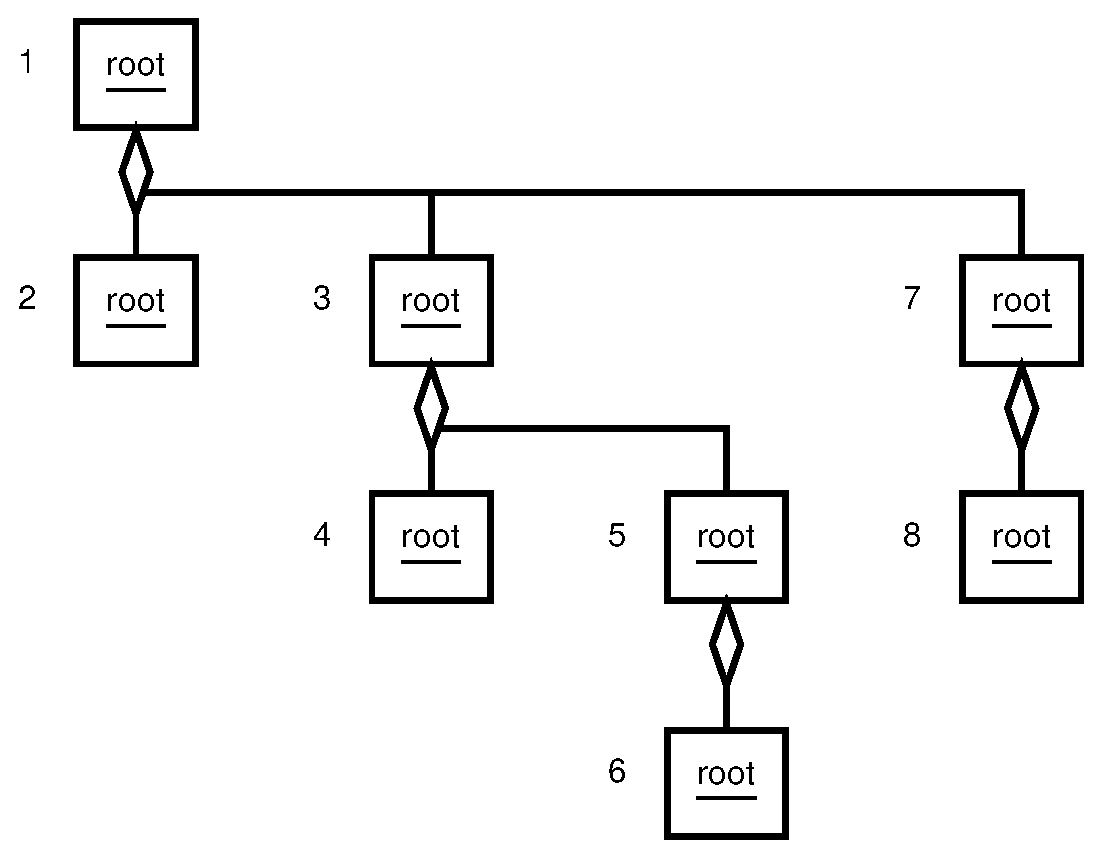
\includegraphics[scale=0.4]{order_root}
\end{center}
\caption{Beispiel: Ordnung der root-Elemente}
\label{figOrderRoot}
\end{figure}

F"ur ein Fib-Objekt sind jeweils alle root-Objekte sichbar, die nach den Fib-Objekten (in root-Elementen) stehen, in denen es enthalten ist, und die root-Objekte, die in der Datenbank stehen.

Soll ein externes Objekt \index{Externe Objekte} in einem Fib-Objekt aufgel"ost werden, werden zuerst die Identifier im n"achsten root-Element durchsucht, in dem das Fib-Objekt enthalten ist, danach im n"achsten root-Element usw. Dabei werden nur Identifier "uberpr"uft, die nach dem Identifier f"ur das root-Objekt kommen, in dem das Fib-Objekt enthalten ist. Das Haupt-Fib-Objekt steht vor allen enthaltenden root-Objekten (mit Identifiern) eines root-Elements. Am Ende werden noch die Datenbankobjekte "uberpr"uft.

\bigskip\noindent
Beispiel: Es sei folgende root-Element-Struktur gegeben:

\begin{eqnarray*}
root_0&=&root( \ldots , Obj_0 , (( 1, root_1), ( 2, root_2), ( 3, root_3)), \ldots )\\
\\
root_1&=&root( \ldots , Obj_1 , (( 11, root_{11})),  \ldots )\\
root_{11}&=&root( \ldots , Obj_{11} , (( 111, root_{111})), \ldots )\\
root_{111}&=&root( \ldots , Obj_{111} , (), \ldots )\\
\\
root_2&=&root( \ldots , Obj_2 , (( 21, root_{21})),  \ldots )\\
root_{21}&=&root( \ldots , Obj_{21} , (), \ldots )\\
\\
root_3&=&root( \ldots , Obj_3 , (( 31, root_{31})),  \ldots )\\
root_{31}&=&root( \ldots , Obj_{31} , (), \ldots )\\
\end{eqnarray*}

Das root-Element $root_0$ ist das Wurzel-root-Element.
Im Folgenden ist f"ur einige Fib-Objekte angegeben, welche Identifier und damit root-Objekte sie in externen Objekten verwenden k"onnen bzw. welche root-Elemente aufgel"ost werden k"onnen bzw. sichtbar sind. (Es wird hier keine Fib-Datenbank ber"ucksichtigt. Root-Objekte der Datenbank w"aren f"ur alle Fib-Objekte sichtbar.) Die Identifier und root-Elemente sind in der Reihenfolge angegeben, wie sie bei der Suche durchlaufen werden.
\begin{itemize}
 \item $Obj_0$: $( 1, root_1)$, $( 2, root_2)$, $( 3, root_3)$
 \item $Obj_1$: $( 11, root_{11})$, $( 2, root_2)$, $( 3, root_3)$
 \item $Obj_{11}$: $( 111, root_{111})$, $( 2, root_2)$, $( 3, root_3)$
 \item $Obj_2$: $( 21, root_{21})$, $( 3, root_3)$
 \item $Obj_{21}$: $( 3, root_3)$
 \item $Obj_3$: $( 31, root_{31})$
 \item $Obj_{31}$: keine
\end{itemize}

\index{root-Element|)}


\section{Die Fib-Datenbank}
\label{secFibDatabase}

Die Fib-Datenbank geh"ort zu keinem Fib-Multimediaobject. Sie wird mit den Fib-Bib\-lio\-the\-ken /dem Fib-System ausgeliefert und enth"alt h"aufig verwendete Datenbankobjekte, die in Fib-Objekten verwendet werden k"onnen. Fib-Objekte k"onnen die Datenbankobjekte verwenden, ohne diese beinhalten zu m"ussen. Datenbankobjekte k"onnen beispielsweise Linien (mit den Eingabeparametern f"ur Start- und Endpunkte), Recht\-ecke oder Kreise sein, aber auch B"aume, Autos, Zeichens"atze (fonts) oder Fraktale. Wird in einem Fib-Objekt beispielsweise ein Kreis ben"otigt, kann dass entsprechende parametrisierte Datenbankobjekt verwendet werden.

Eine detailierte Beschreibung der Fib-Datenbank kann in Teil \ref{partFibDatabase} auf Seite \pageref{partFibDatabase} gefunden werden.

Die Implementierung der Datenbankobjekte kann an die jeweilige Anwendungsumgebung angepasst sein. Soll zur Anzeige beispielsweise OpenGL verwendet werden, k"onnen Datenbankobjekte direkt mit OpenGL-Primitiven (z. B. Dreiecken) umgesetzt werden. Auf diese Weise kann mit Datenbankobjekten die Performance der Anwendung verbessert werden. Bei der Kodierung der Fib-Objekte kann auch gleich darauf geachtet werden, dass Datenbankobjekte mit guter Performance f"ur die Zielanwendung verwendet werden. Diese Fib-Objekte sind dann immer noch auf allen Fib-Systemen mit gen"ugend hoher Datenbankversion anzeigbar, auf einigen jedoch schneller.

Welche Objekte eine Datenbank enth"alt, sowie die Identifier f"ur diese Objekte, sind mit der Datenbankversion festgelegt. Datenbanken mit h"oheren Datenbankversionen enthalten dabei alle Datenbankobjekte mit den gleichen Identifiern wie Datenbanken mit niedrigeren Datenbankversionen. Auf diese Weise ist gew"ahrleistet, dass Fib-Objekte immer aufw"artskompatibel zu neueren Datenbankversionen sind.

Alle Identifier von Datenbankobjekten sind negativ.



\section{Definitionen f"ur Fib}
\label{secDefinitionsForFib}

In diesem Abschnitt werden einige Definitionen f"ur die Fib-Multimediasprache gegeben. Diese sollen den Umgang mit und das Verst"andnis f"ur Fib erleichtern.

\subsection{Definition des korrekten Fib-Objekt}

Ein \textbf{Fib-Objekt} ist korrekt, wenn es der oben aufgef"uhrten Fib-Syntax entspricht, alle Variablen, die es enth"alt, "uber es definiert sind und jedes enthaltende Fib-Element in ihm ein korrektes Fib-Element ist. Zu einem korrekten Fib-Objekt muss ein korrektes root-Element geh"oren. Damit ein Fib-Element korrekt ist, muss es zu seinem root-Element passen (das hei"st unter Anderem korrekte [Anzahl von] Dimensionen und Definitionsbereiche).

Korrekte Fib-Objekte werden auch kurz nur als Fib-Objekte bezeichnet.

\bigskip\noindent
Ein \textbf{Fib-Element} entspricht der oben vorgestellten Fib-Syntax, au"ser dass keine Fib-Elemente in ihm enthalten sind bzw. betrachtet werden.

\bigskip\noindent
In den nachfolgenden Beispielen werden Kommentare mit ``//'' eingeleitet. Diese geh"oren nicht mehr zu den dargestellten Fib-Elementen.

\begin{flushleft}
Beispiele:\\
Korrekte Fib-Objekte (Es wird angenommen, dass das zugeh"orige root-Element korrekt und passend ist.):
\begin{eqnarray*}
Obj &=& pr( (3)_{colorGrayscale}, p((1;5)))\\
Obj &=& list( for(y,[(4;2)], pr( (3, 42, 125)_{colorRGB} , p((7;y))), \\
&& fun(x,add( mult(4, exp( 3, -2)), 2 ), pr( (205, x ,x)_{colorRGB}, p((3;x)) ) )\\
\end{eqnarray*}

Fib-Element ($Elm$):
\begin{eqnarray*}
Elm &=& p((3;2;5)) \textnormal{//3-dimensional}\\
Elm &=& for(x,[(3;8)],null) \\
& & \textnormal{//null ist kein Objekt (bei der Implementierung ein Nullzeiger)}\\
Elm &=& p((2;5))\\
\end{eqnarray*}

Weder ein Fib-Element noch ein korrektes Fib-Objekt ($Woe$ ; $null$ ist kein Objekt [bei der Implementierung Nullzeiger]) :\\
\begin{eqnarray*}
Woe &=& list( for( x, [(3;7)], null), null)\\
Woe &=& fun( x, add(4, exp(6, 3) ) , for(y, [(6;7)], null))\\
Woe &=& pr( (3)_{colorRGB}, p((1;5)) ): \textnormal{//ung"ultige Syntax des} \\
&& \textnormal{Eigenschaftselements: Der colorRGB-Vektor verlangt}\\
&& \textnormal{nach 3 Parametern.}\\
\end{eqnarray*}

\end{flushleft}


\subsection{Definition des vollst"andigen Fib-Objekt}
\label{secFullFibObject}

Ein vollst"andiges Fib-Objekt ist ein Fib-Objekt, welches ein darstellbares Multimediaobjekt repr"asentiert. Jedes vollst"andige Fib-Objekt ist auch ein korrektes Fib-Objekt. Zum vollst"andigen Fib-Objekt geh"oren unter Anderem alle notwendigen root-Elemente mit den Angaben der richtigen Fib- und Datenbankversion.


\subsection{Definition von ``unterhalb'' und ``oberhalb'' in einem Fib-Objekt}
\label{secDefinitionUpDown}

Man stelle sich ein Fib-Objekt als Baum vor, in dem die Root und Listenelemente die Verzweigungen darstellen.
Da in der Informatik im Allgemeinen die Wurzel oben dargestellt wird, sind die Elemente, welche das Element $Elm$ enth"alt, unten und die Elemente, welche das Element $Elm$ enthalten, f"ur dieses oben.

Unterhalb eines Elements $Elm$ bedeutet also, dass die Elemente gemeint sind, die das Element $Elm$ direkt oder indirekt enthalten.
Demgegen"uber sind oberhalb eines Elements $Elm$, die Elemente, die das Element $Elm$ direkt oder indirekt, enthalten.

Dieser Sachverhalt ist in Abbildung \ref{figDirectionFibElements} dargestellt. Das Listenelement in der Mitte, das mit 1 gekennzeichnet ist, ist das Element bez"uglich dessen oberhalb und unterhalb bestimmt wird.

\begin{figure}[htbp]
\begin{center}
  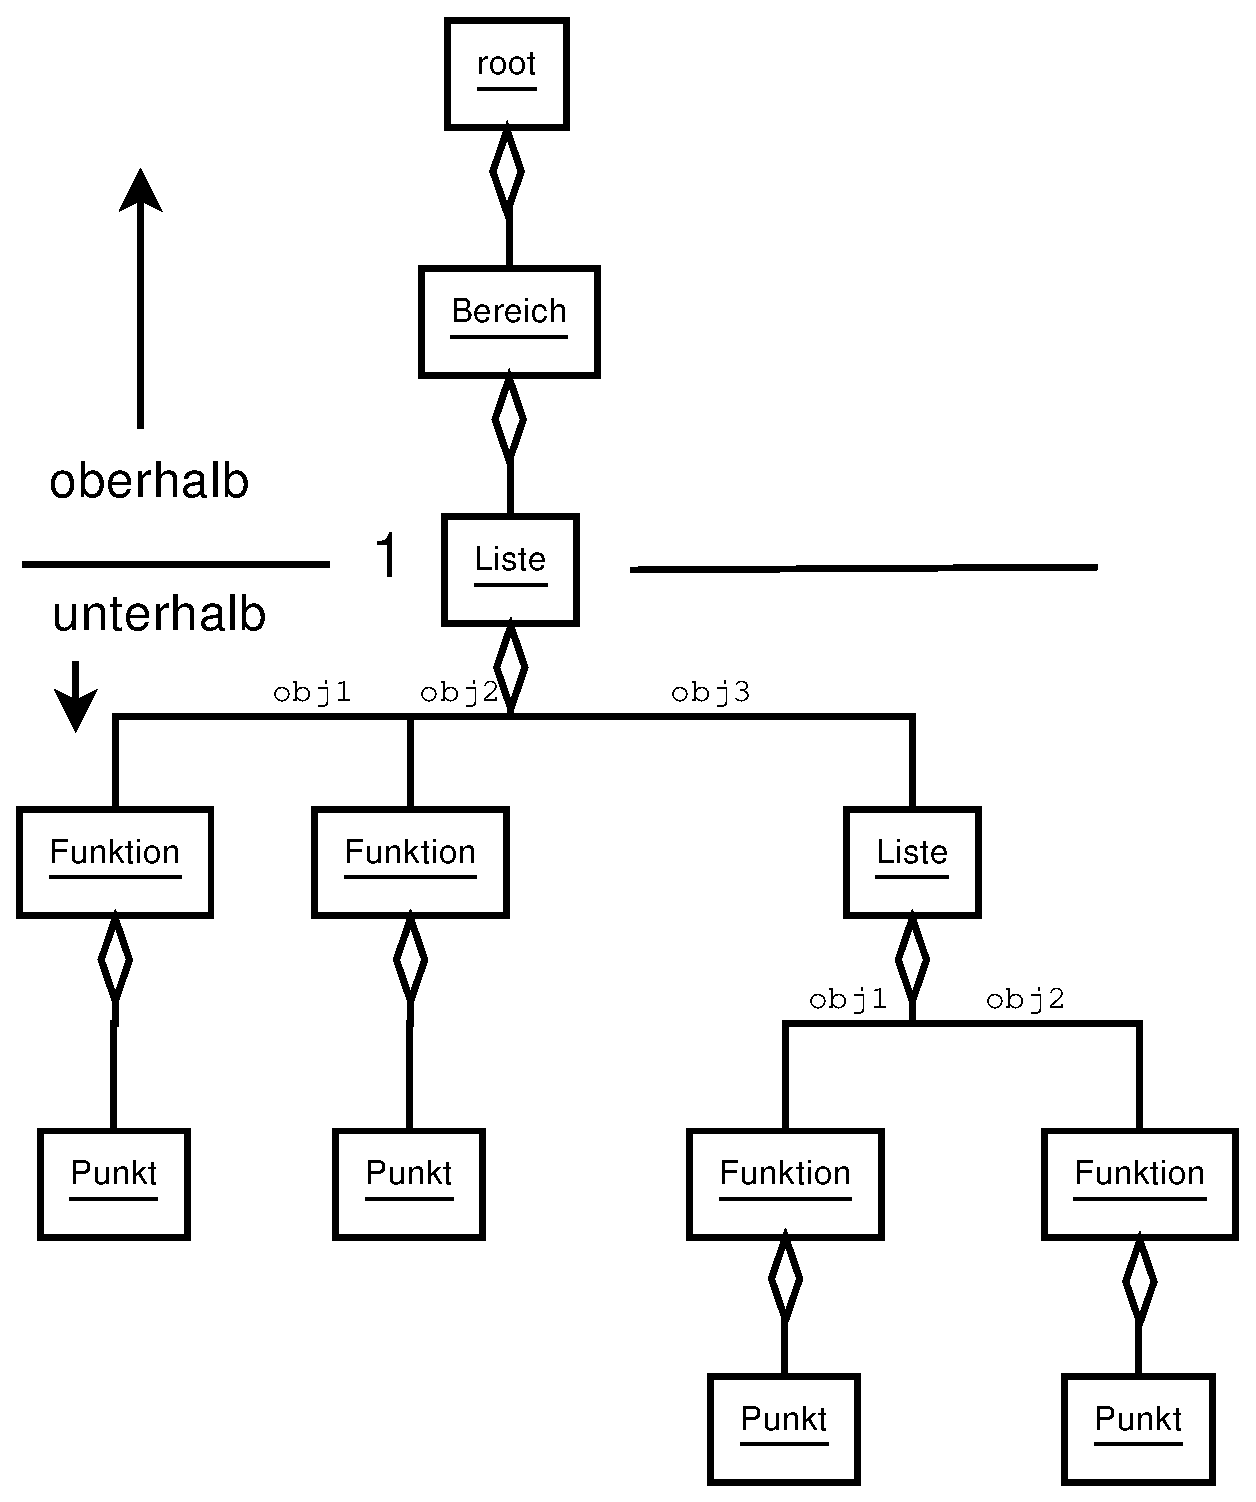
\includegraphics[scale=0.5]{oberhalb_unterhalb}
\end{center}
\caption{Beispiel f"ur oberhalb und unterhalb in einem Fib-Objekt}
\label{figDirectionFibElements}
\end{figure}


\subsection{Ordnung der Fib-Elemente}\index{Ordnung!Fib-Elemente}
\label{secOrderFibElements}

Auf den Definitionen von ``unterhalb'' und ``oberhalb'' in einem Fib-Objekt wird die Ordnung der Fib-Elemente aufgebaut. Jedem Fib-Element im vollst"andige Fib-Objekt wird eine eindeutige nat"urliche Zahl zugeordnet. Wenn in einem Fib-Objekt $N$ Elemente existieren, werden den Fib-Elementen im Fib-Objekt die Zahlen $1$ bis $N$ zugeordnet. Fib-Elementen unterhalb eines Fib-Elements werden h"ohere Werte zugeordnet.

Bei Listenelementen haben Unterobjekte $Obj_U$ des Listenelements mit einer h"oheren Nummer $U$ als ein anderes Unterobjekt $Obj_K$ ($U>K$) auch h"ohere Nummern f"ur ihre enthaltenden Elemente, als die Elemente in $Obj_K$. Die root-Elemente werden in der Ordnung genauso behandelt wie Listenelemente, wobei das Haupt-Fib-Objekt das erste Unterobjekt ist, dem die Unter-root-Objekte in ihrer Reihenfolge (im root-Element) folgen.

Das selbe gilt f"ur alle anderen Zweigelemente. Die oben vorgestellte Syntax gibt dabei die Reihenfolge der Unterobjekte vor.

In Abbildung \ref{figOrderFibElements} ist eine Beispielobjekt mit den zugeh"origen Zahlen (links neben den Elementen) der Ordnung der Fib-Element dargestellt.

\begin{figure}[htbp]
\begin{center}
  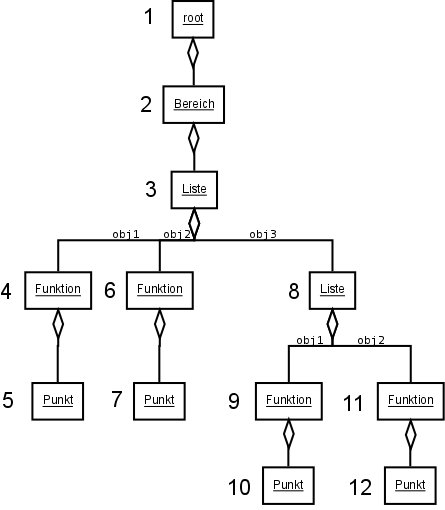
\includegraphics[scale=0.5]{order_elements}
\end{center}
\caption{Beispiel f"ur die Ordnung der Fib-Elemente}
\label{figOrderFibElements}
\end{figure}


\subsection{Ordnung bestimmter Fib-Elemente}\index{Ordnung!bestimmte Fib-Elemente}

Auch Fib-Elemente eines bestimmten Typs sind nat"urliche Zahlen einer Ordnung zugeordnet. Diese Ordnungen orientieren sich an der Ordnung der Fib-Elemente. Wenn in einem korrekten Fib-Objekt $N$ Fib-Elemente eines Typs existieren, so sind den Fib-Elementen dieses Typs die Zahlen $1$ bis $N$ zugeordnet. Ist ein Fib-Element $Elm_1$ in der Ordnung der Fib-Elemente ein h"oherer Wert zugeordnet (als einem anderen Fib-Element $Elm_2$ des gleichen Typs), so ist ihm ($Elm_1$) auch in der Ordnung der Fib-Elemente des gleichen Typs ein h"oherer Wert zugeordnet (als dem anderen Fib-Element $Elm_2$).

In Abbildung \ref{figOrderSpecialFibElements} ist eine Beispielobjekt mit den zugeh"origen Zahlen (links neben den Elementen) der Ordnungen der einzelnen Fib-Element dargestellt.

\begin{figure}[htbp]
\begin{center}
  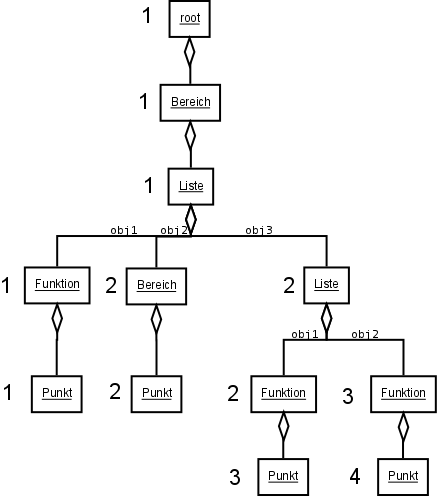
\includegraphics[scale=0.5]{order_special_elements}
\end{center}
\caption{Beispiel f"ur die Ordnung bestimmter Fib-Elemente}
\label{figOrderSpecialFibElements}
\end{figure}


\subsection{Ordnung der Verschiebungspunkte}\index{Verschiebungspunkte}\index{Ordnung!Verschiebungspunkte}

Eine weitere Ordnung betrifft alle Fib-Elemente, die verschoben werden k"onnen. Diese werden Verschiebungspunkte genannt.
Die Ordnungen der Verschiebepunkte orientieren sich an der Ordnung der Fib-Elemente. Wenn in einem vollst"andigen Fib-Objekt $N$ Verschiebepunkte existieren, so sind den Verschiebepunkte, die Zahlen $1$ bis $N$ zugeordnet. Ist ein Fib-Element in der Ordnung der Fib-Elemente ein h"oherer Wert zugeordnet, so ist ihm auch in der Ordnung der Verschiebepunkte ein h"oherer Wert zugeordnet.

\bigskip\noindent
Fib-Elemente, welche verschoben werden k"onnen und Verschiebepunkte darstellen, sind alle Zweigelemente (limb Elemente; sie enthalten genau ein Unterobjekt):
\begin{itemize}
 \item Eigenschaftselement (siehe Abschnitt \ref{fibProperty} auf Seite \pageref{fibProperty})
 \item Anmerkungselemente (siehe Abschnitt \ref{fibComment} auf Seite \pageref{fibComment})
 \item Bereichselemente (siehe Abschnitt \ref{fibArea} auf Seite \pageref{fibArea})
 \item Funktionselemente (siehe Abschnitt \ref{fibFunction} auf Seite \pageref{fibFunction})
 \item Fib-Element, um Definitionsbereichseigenschaften abzurufen (siehe Abschnitt \ref{fibDomeinProperties} auf Seite \pageref{fibDomeinProperties})
 \item Set-Element (siehe Abschnitt \ref{secFibSetElement} auf Seite \pageref{secFibSetElement})
 \item Matrixelement (siehe Abschnitt \ref{secFibMatrixElement} auf Seite \pageref{secFibMatrixElement})
\end{itemize}

\bigskip\noindent
Fib-Elemente, welche nicht verschoben werden k"onnen und damit keine Verschiebepunkte darstellen, sind:
\begin{itemize}
 \item Alle Blattelemente:
 \begin{itemize}
  \item Punkte (siehe Abschnitt \ref{fibPoint} auf Seite \pageref{fibPoint})
  \item Fib-Elemente f"ur externe Unterobjekte (siehe Abschnitt \ref{fibSubobject} auf Seite \pageref{fibSubobject})
 \end{itemize}
 \item Alle Verzweigungselemente:
 \begin{itemize}
  \item Root-Element (siehe Abschnitt \ref{fibRootElement} auf Seite \pageref{fibRootElement})
  \item Listenelement (siehe Abschnitt \ref{fibList} auf Seite \pageref{fibList})
  \item Das Fib-Element, um externe Objekte aufzurufen (siehe Abschnitt \ref{fibExtObject} auf Seite \pageref{fibExtObject})
  \item Bedingungen mit dem if-Element (siehe Abschnitt \ref{secFibIf} auf Seite \pageref{secFibIf})
 \end{itemize}
\end{itemize}

In Abbildung \ref{figOrderMovePoints} ist ein Beispielobjekt mit den zugeh"origen Zahlen (links neben den Elementen) der Ordnung der Verschiebepunkte dargestellt.

\begin{figure}[htbp]
\begin{center}
  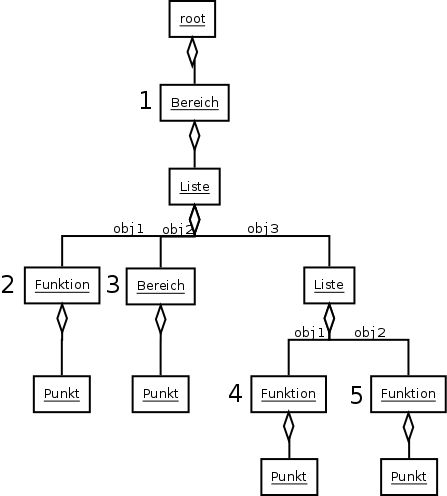
\includegraphics[scale=0.5]{order_move_points}
\end{center}
\caption{Beispiel f"ur die Ordnung der Verschiebungspunkte}
\label{figOrderMovePoints}
\end{figure}


\subsection{Definition Teilobjekt}\index{Teilobjekt|(}

Jedes Objekt, das ein ganzer Zweig (z. B. Unterlistenobjekt, Haupt-Fib-Objekt oder Unter-root-Objekt) eines Verzweigungselements ist, ist Teil eines Teilobjekts. Weiterhin geh"oren zum Teilobjekt alle root-Elemente, in denen es enthalten ist oder die es "uber externe Objekte benutzt. Auch Fib-Elemente, die Variablen definieren, welche in dem Teilobjekt verwendet werden, geh"oren dazu.
Die Vereinigung zweier Teilobjekte ist wieder ein Teilobjekt.
Das ganze Fib-Objekt selbst ist auch ein Teilobjekt.
Ein Teilobjekt kann immer zu einem Multimediaobjekt ausgewertet werden.

Ein \textbf{echtes Teilobjekt}\index{Teilobjekt!echtes} ist ein Teilobjekt, das nicht das (ganze) Fib-Objekt selbst ist.

Ein \textbf{einfaches Teilobjekt}\index{Teilobjekt!einfach} ist ein echtes Teilobjekt, das nur ein Blatt mit einem Punktobjekt enth"alt.

Ein \textbf{zusammenh"angendes Teilobjekt}\index{Teilobjekt!zusammenh"angendes} ist ein echtes Teilobjekt, welches das gesamte Objekt eines Arms, genau eines Verzweigungselements (z. B. Listenelements oder root-Elements) enth"alt und die ben"otigten Elemente "uber diesem. Insbesondere ist jedes einfache Teilobjekt ein zusammenh"angendes Teilobjekt.

Um ein zusammenh"angendes Teilobjekt zu erzeugen, kann aus dem ganzen Fib-Objekt ein Verzweigungselement (z. B. Listenelement oder root-Element) gel"oscht und durch ein in ihm enthaltendes Unterobjekt ersetzt werden. Das erzeugte Teilobjekt muss nat"urlich korrekt sein, um ein zusammenh"angendes Teilobjekt zu sein. (Es darf beispielsweise bei einem root-Element nicht das Haupt-Fib-Objekt gel"oscht werden, und wenn ein root-Element gel"oscht wird, und das n"achste Haupt-Fib-Objekt oberhalb durch sein Haupt-Fib-Objekt ersetzt wird, m"ussen die Definitionsbereiche des ersetzten root-Elements vom n"achsten enthaltenden root-Element "ubernommen werden.)

Mit Abbildung \ref{figOrderFibElementsPartobjects} sei diese Definition an einem Beispiel eines Fib-Objekts dargestellt. Im Nachfolgenden werden einige Beispiele f"ur unterschiedliche Typen von Teil\-objekte in Abbildung \ref{figOrderFibElementsPartobjects} gegeben, wobei f"ur die Fib-Elemente ihre Nummern (aus der Fib-Elementordnung bzw. der Abbildung \ref{figOrderFibElementsPartobjects}) angegeben werden. Weiterhin wird festgelegt, dass das Punktelement mit der Nummer $10$ nicht die Variable benutzt, welche das Bereichselement mit der Nummer $2$ definiert. Alle anderen Variablen werden in den Punkten ben"otigt, welche unter der jeweiligen Variablendefinition stehen.

\begin{figure}[htbp]
\begin{center}
  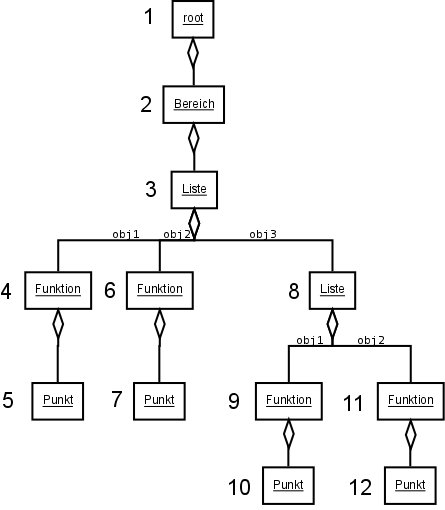
\includegraphics[scale=0.5]{order_elements}
\end{center}
\caption{Beispiel Objekt f"ur Teilobjekte}
\label{figOrderFibElementsPartobjects}
\end{figure}


\bigskip\noindent
Teilobjekte:
\begin{itemize}
 \item 1; 2; 4; 5
 \item 1; 2; 6; 7
 \item 1; 2; 3 (nur Unterobjekt $1$ und $2$); 4; 5; 6; 7
 \item 1; 9; 10
 \item 1; 2; 8; 9; 10; 11; 12
 \item 1; 2; 3 (nur Unterobjekt $1$ und $3$); 4; 5; 8; 9; 10; 11; 12
 \item 1; 2; 3 (nur Unterobjekt $1$ und $3$); 4; 5; 11; 12
 \item (alle Fib-Elemente) 1; 2; 3; 4; 5; 6; 7; 8; 9; 10; 11; 12
\end{itemize}

Echte Teilobjekte:
\begin{itemize}
 \item 1; 2; 4; 5
 \item 1; 2; 6; 7
 \item 1; 2; 3 (nur Unterobjekt $1$ und $2$); 4; 5; 6; 7
 \item 1; 9; 10
 \item 1; 2; 8; 9; 10; 11; 12
 \item 1; 2; 3 (nur Unterobjekt $1$ und $3$); 4; 5; 8; 9; 10; 11; 12
 \item 1; 2; 3 (nur Unterobjekt $1$ und $3$); 4; 5; 11; 12
\end{itemize}

Einfache Teilobjekte:
\begin{itemize}
 \item 1; 2; 4; 5
 \item 1; 2; 6; 7
 \item 1; 9; 10
 \item 1; 2; 11; 12
\end{itemize}

Zusammenh"angende Teilobjekte:
\begin{itemize}
 \item 1; 2; 4; 5
 \item 1; 2; 6; 7
 \item 1; 9; 10
 \item 1; 2; 11; 12
 \item 1; 2; 8; 9; 10; 11; 12
\end{itemize}


\subsection{Die Ordnung der zusammenh"angenden Teilobjekte}
\label{secOrderPartobjects}

Auch auf den zusammenh"angenden Teilobjekten gibt es eine Ordnung. Diese wird im Nachfolgenden auch Ordnung der Teilobjekte gennant, da es f"ur die anderen Arten von Teilobjekten keine eigene Ordnung gibt.

Die Ordnungen der (zusammenh"angenden) Teilobjekte orientieren sich an der Ordnung der Fib-Elemente. Wenn in einem vollst"andigen Fib-Objekt $N$ zusammenh"angende Teilobjekte existieren, so sind den zusammenh"angenden Teilobjekten die Zahlen $1$ bis $N$ zugeordnet.
Je gr"o"ser die Nummer eines zusammenh"angenden Teilobjekts ist, desto gr"o"ser ist auch die kleinste Nummer in Ordnung der Fib-Elemente, der Fib-Elemente in ihm.
%Ist einem Fib-Element in der Ordnung der Fib-Elemente ein h"oherer Wert zugeordnet, so ist dem Teilobjekt, welches unter den Teilobjekten, die das Fib-Element enth"alt, die gr"o"ste Nummer in der Ordnung der Teilobjekte hat, auch in der Ordnung der zusammenh"angenden Teilobjekt ein h"oherer Wert zugeordnet.
Oder auch: Ist dem obersten Fib-Element des Unterobjekts, "uber das ein zusammenh"angendes Teilobjekt definiert ist, ein h"oherer Wert zugeordnet, so ist auch dem definierten Teilobjekt ein h"oherer Wert zugeordnet.

In Abbildung \ref{figOrderPartobjekts} ist ein Beispielobjekt mit den zugeh"origen Zahlen (links neben den definierenden Unterobjekten der Teilobjekte) in der Ordnung der Teilobjekte dargestellt.

\begin{figure}[htbp]
\begin{center}
  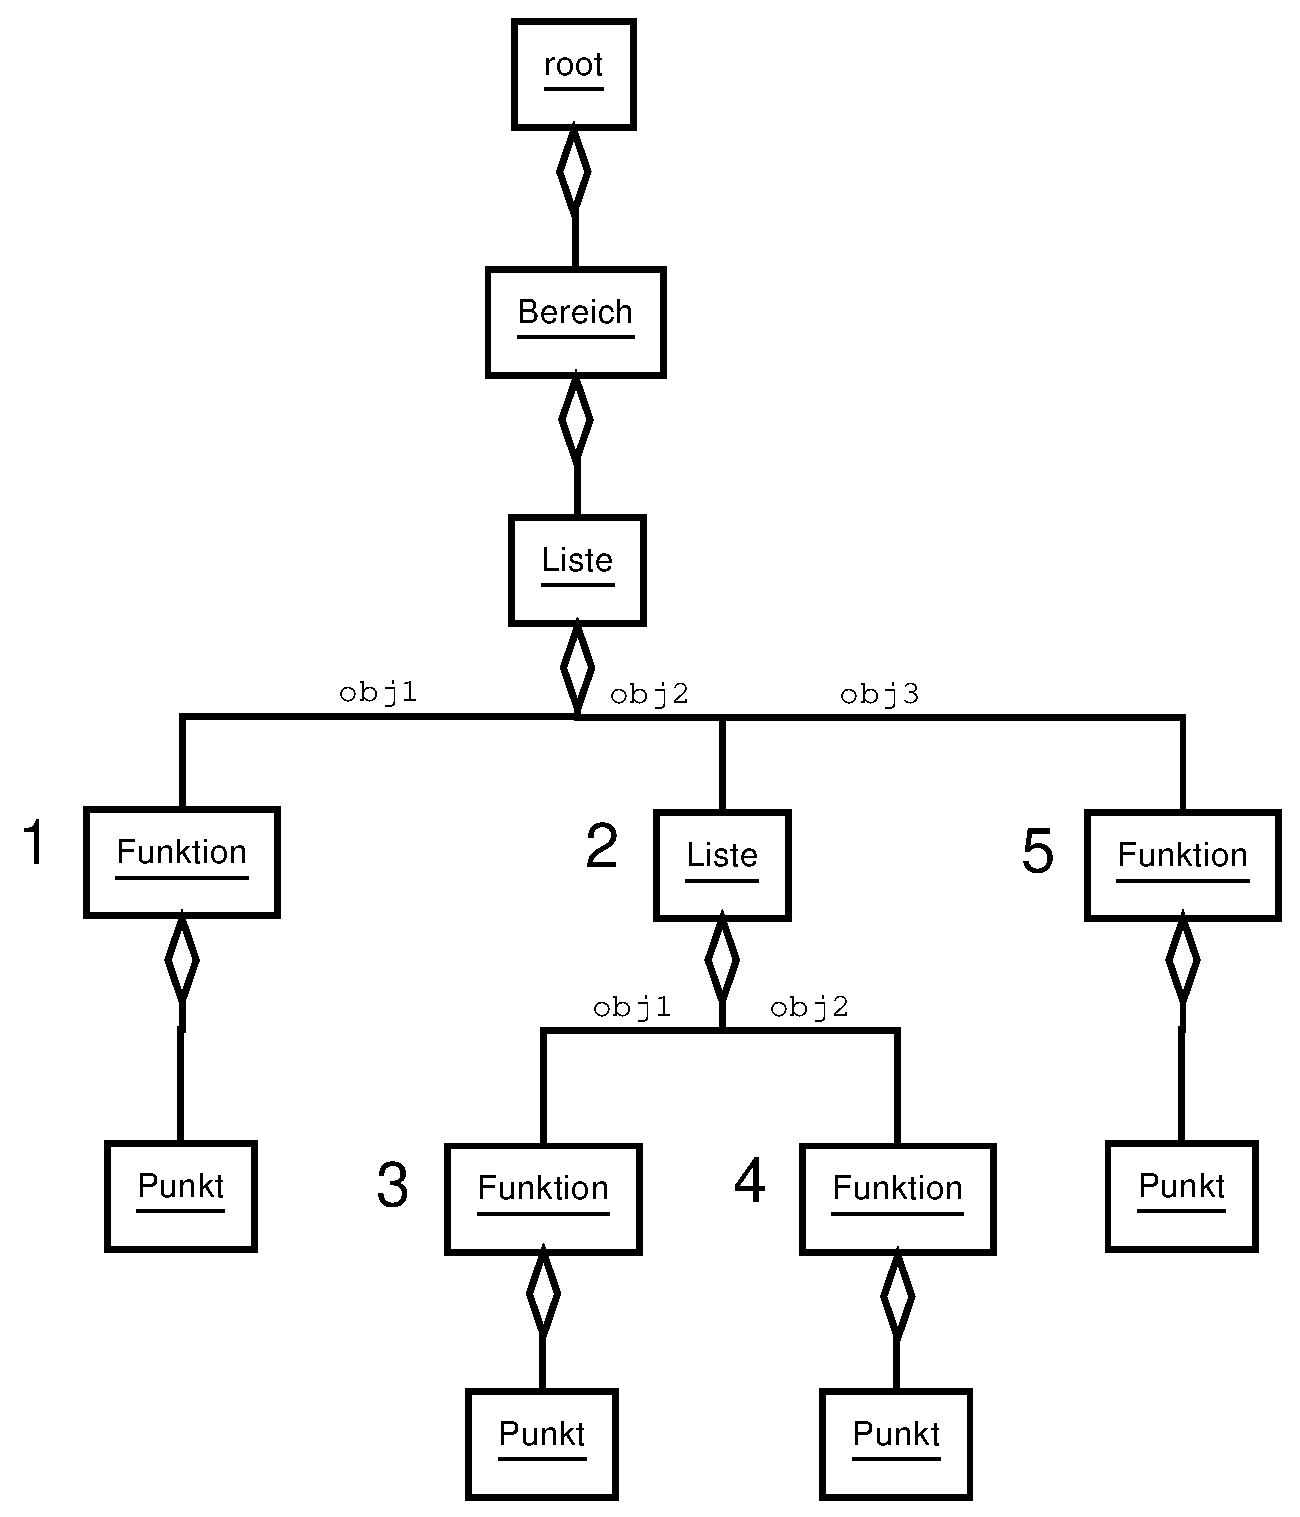
\includegraphics[scale=0.5]{order_partobjects}
\end{center}
\caption{Beispiel f"ur die Ordnung der zusammenh"angenden Teilobjekte}
\label{figOrderPartobjekts}
\end{figure}


\index{Teilobjekt|)}

\subsection{Definition Fib-Multimediaobjekt}\index{Fib-Multimediaobjekt}

Wird der Ausdruck Fib-Multimediaobjekt benutzt, ist damit ein Fib-Objekt mit Schwerpunkt auf dem Multimediaobjekt, das es repr"asentiert, gemeint.


\subsection{Definition richtiges Fib-Multimediaobjekt}\index{Fib-Multimediaobjekt!richtiges}

Ein richtiges Fib-Multimediaobjekt ist ein Fib-Objekt, welches das originale Multimediaobjekt, das es repr"asentieren soll, vollst"andig wiedergibt. Wenn also das Multimediaobjekt, welches das Fib-Objekt repr"asentiert, und das originale Multimediaobjekt verglichen werden, kann kein Unterschied zwischen ihnen feststellt werden.



%TODO: in welche Sprache kontextfrei oder regul"ar?



